\chapter{Pengembangan Dan Pengujian}

\par Pada tugas akhir ini, perangkat lunak yang dikembangan berupa sistem manajemen kompetisi, \textit{autograder} dan program antar muka pengguna.  Sistem manajemen kompetisi di-\textit{deploy} pada komputer yang disediakan oleh juri dan bertindak sebagai \textit{server}. \textit{Autograder} dan program antar muka akan didistribusikan kepada peserta dan juri untuk dijalankan pada komputernya. Secara keseluruhan, perangkat lunak yang dikembangkan dinamakan UGrade. Nama tersebut berasal dari kata \textit{you} dan \textit{grade}. Nama tersebut dipilih karena proses penilaian atau \textit{grading} dilakukan oleh masing-masing peserta.

\par Terdapat tiga program utama yang dikembangkan pada UGrade yaitu: UGServer, UGJob dan UGDesktop. UGServer berfungsi sebagai sistem manajemen kompetisi yang bertindak sebagai server. UGJob berfungsi sebagai \textit{worker} dari \textit{autograder}. UGDesktop berfungsi sebagai antar muka antara pengguna dengan sistem \textit{online judge}. Selain tiga program utama tersebut, terdapat program lain yang digunakan untuk membantu proses pengembangan. Untuk melakukan \textit{sandboxing}, dikembangan program yang bernama UGSbox. Selain itu, untuk memudahkan proses testing, dikembangankan program UGCtl yang dapat digunakan sebagai antar muka pengguna dalam bentuk \textit{command-line}.

\section{UGServer (Sistem Manajemen Kompetisi)}

\par UGServer merupakan sistem manejem kompetisi yang berfungsi untuk mengatur keberjalanan kompetisi. UGServer memberikan layanan kepada peserta dan juri untuk berinteraksi dengan kompetisi. Layanan yang diberikan oleh UGServer antara lain:
\begin{enumerate}
  \item Otentikasi dan otorisasi pengguna.
  \item Pembuatan dan pengaksesan kompetisi.
  \item Pembuatan dan pengaksesan soal pada kompetisi.
  \item Pengiriman dan pengaaksesan jawaban pada kompetisi.
\end{enumerate}

\par Sebenarnya masih banyak layanan lain yang harus diberikan oleh sistem manajemen kompetisi. Akan tetapi, tugas akhir ini lebih difokuskan pada pengembangan \textit{autograder} dibandingkan dengan sistem manajemen kompetisi. Hal ini dikarenakan tujuan dari tugas akhir ini lebih berfokus pada proses penilaian jawaban peserta. Oleh karena itu, fungsionalitas yang dipaparkan pada paragraf di atas sudah cukup untuk memenuhi tujuan dari tugas akhir ini.

\par UGServer dikembangkan dengan menggunakan \textit{framework django}. Pengembangan perangkat lunak berbasis \textit{web} dapat dengan cepat dan mudah dilakukan menggunakan \textit{framework django}. Kemudahan dan kecepatan pengembangan tersebut disebabkan karena \textit{django} telah memberikan banyak fitur yang sangat membantu proses pengembangan perangkat lunak seperti otorisasi, otentikasi, dan ORM (\textit{object relational mapper}). Terdapat beberapa teknologi alternatif lain yang dapat digunakan dan dapat meningkatkan kinerja sistem manajemen kompetisi seperti Express atau Go. Kedua alternatif tersebut tidak digunakan karena membutuhkan waktu pengembangan yang lama dan tidak memberikan peningkatan kinerja yang signifikan. Oleh karena itu, \textit{framework} \textit{django} dipilih untuk mengembangkan UGServer karena mudah dan cepat untuk dikembangkan.

\par UGServer memberikan API (\textit{application programming interface}) yang dapat digunakan oleh pengguna. API yang diberikan oleh UGServer berupa GraphQL yang berjalan di atas protokol HTTP. GraphQL digunakan karena mudah untuk diimplementasikan dan digunakan. UGDesktop dan UGCtl merupakan program antar muka pengguna yang menggunakan API ini. Terdapat beberapa alternatif lain yang dapat digunakan untuk mengembangkan API dari UGServer seperti menggunakan arsitektur REST (\textit{representational state transfer}) atau menggunakan RPC (\textit{remote procedure call}). Alternatif tersebut tidak digunakan karena tidak fleksibel dan sulit untuk diimplementasikan.

\begin{figure}[ht!]
    \centering
    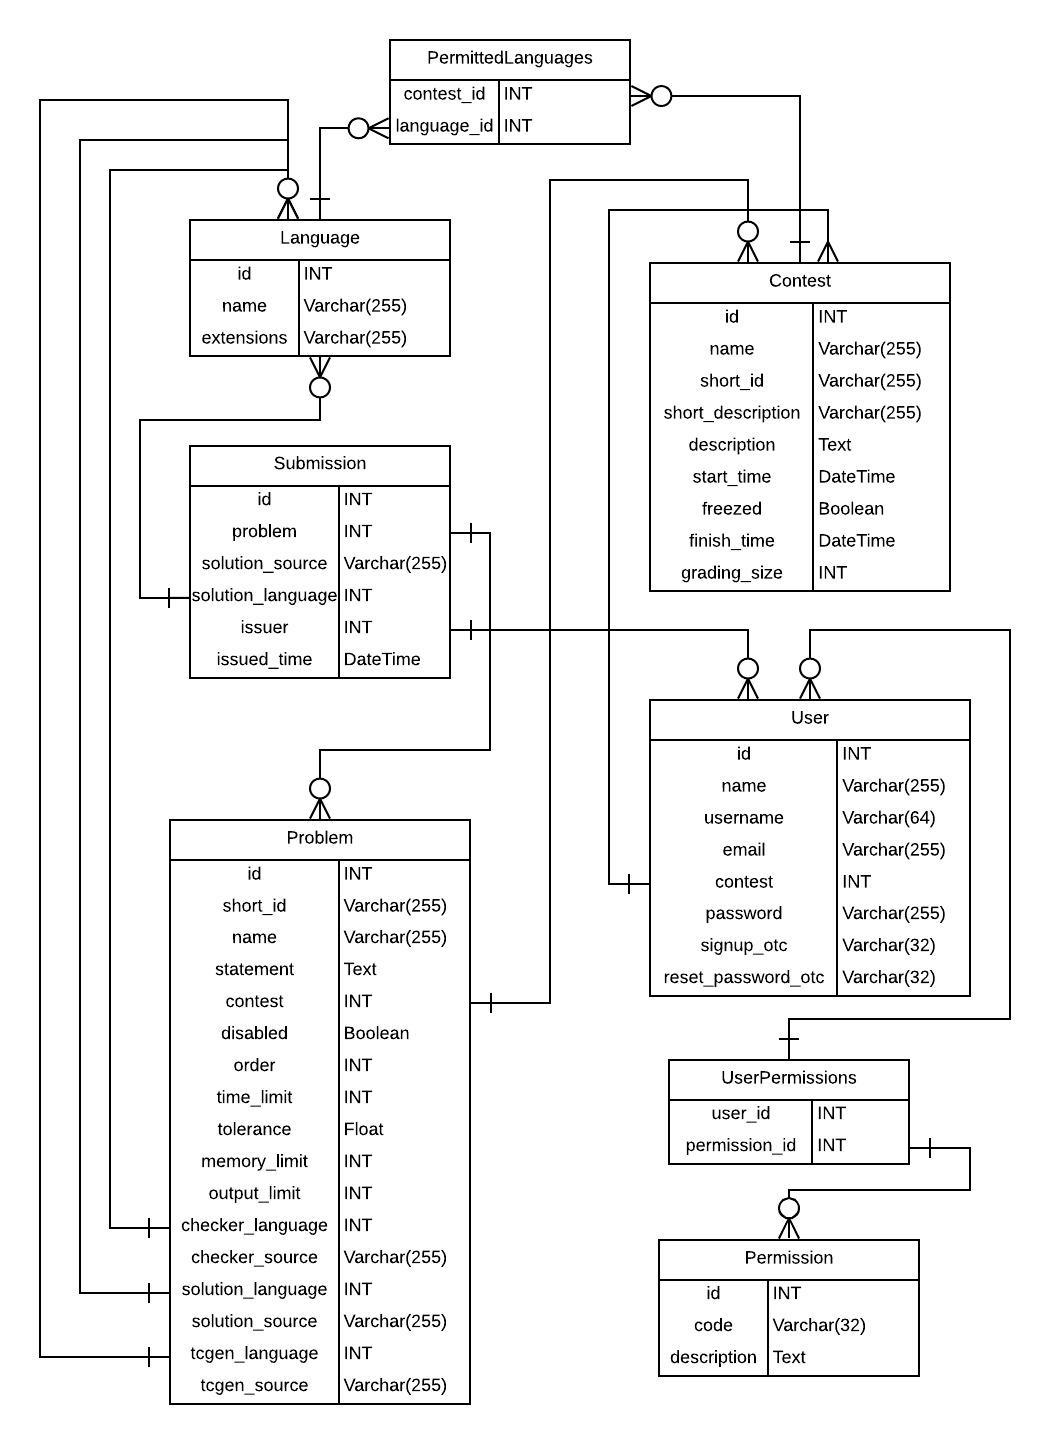
\includegraphics[width=0.8\textwidth]{images/dbschemas}
    \caption{Skema Basis Data Sistem Manajemen Kompetisi}
    \label{fig:dbschemas}
\end{figure}

\par Dalam menjalankan fungsinya, UGServer menggunakan sistem manajemen basis data untuk menyimpan informasi terkait kompetisi. Pada saat ini, UGServer dapat berjalan menggunakan sistem basis data Postgresql atau SQLite. \textit{Framework django} memiliki fitur ORM yang siap digunakan untuk basis data yang bersifat relasional. Karena adanya fitur tersebut, data lebih mudah untuk diatur menggunakan basis data relasional. Oleh karena itu, pada tugas akhir ini penyimpanan data dilakukan dengan memanfaatkan sistem basis data relasional. Gambar \ref{fig:dbschemas} merupakan skema basis data yang digunakan untuk menyimpan informasi terkait kompetisi.

\subsection{Manajemen Pengguna} \label{subsec:user-management}

% akun
\par UGServer memberikan layanan untuk melakukan manajemen pengguna. Pengguna pada UGrade terikat pada suatu kompetisi. Pengguna pada suatu kompetisi tidak dapat mengikuti kompetisi lain. Pengguna yang ingin mengikuti dua buah kompetisi harus membuat dua akun. Pengguna dapat membuat akun dengan cara membuat kompetisi. Ketika seseorang membuat kompetisi, maka sebuah akun akan tercipta sesuai dengan alamat \textit{email} orang tersebut. Selain itu, akun dapat dibuat dengan mengundang orang lain ke dalam kompetisi.

% otentikasi
\par Akun yang pertama kali dibuat hanya mengandung informasi alamat \textit{email} pengguna dan kode untuk otentikasi. Kode tersebut akan dikirim ke \textit{email} pengguna. Hal ini berfungsi sebagai cara untuk mengotentikasi pengguna dengan cara mengotentikasi \textit{email} pengguna. Pengguna kemudian harus memasukkan kode tersebut untuk mengotentikasi dirinya. Pengguna yang telah terotentikasi akan memasukkan informasi mengenai nama lengkap, \textit{username} dan kata sandi. Nama lengkap merupakan nama yang akan ditampilkan pada antar muka kompetisi. \textit{Username} merupakan nama pengguna yang unik untuk setiap kontes dan bersifat mudah untuk dibaca oleh manusia. Setelah melakukan otentikasi \textit{email}, pengguna selanjutnya dapat melakukan otentikasi dengan kombinasi kompetisi yang diikuti, alamat \textit{email} dan kata sandi yang dipilih. 

% emai + username unik untuk setiap kompetisi
\par Setiap pengguna dalam suatu kompetisi memiliki alamat \textit{email} dan \textit{username} yang unik. Dalam dua kompetisi berbeda bisa saja terdapat akun dengan alamat \textit{email} yang sama. Hal ini dikarenakan akun pengguna terikat pada suatu kompetisi sehingga seorang pengguna dapat diidentifikasi dengan menggunakan informasi kompetisi yang diikutinya dan alamat \textit{email} atau \textit{username}-nya.

\begin{figure}[ht!]
    \centering
    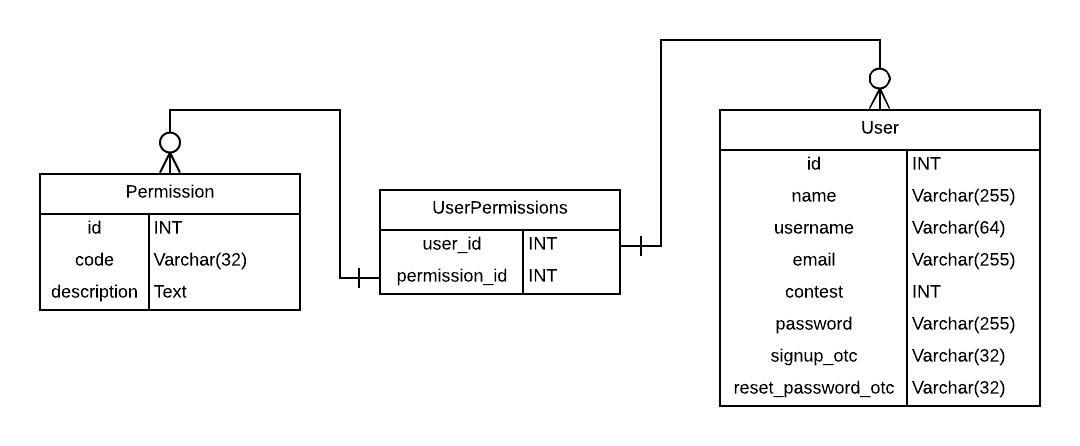
\includegraphics[width=\textwidth]{images/user-schema}
    \caption{Skema Basis Data Sistem Manajemen Pengguna}
    \label{fig:user-schema}
\end{figure}

% user permissions
Pengguna dalam perangkat lunak ini umumnya meliputi juri, peserta dan admin. Perangkat lunak UGServer sebenarnya tidak membeda-bedakan pengguna sebagai juri, peserta ataupun admin. Otorisasi dilakukan dengan memberikan label \textit{permission} kepada setiap pengguna yang ada. Setiap pengguna memiliki himpunan \textit{permission} yang menandakan aksi-aksi apa saja yang dapat dilakukan. Pada saati ini, terdapat beberapa \textit{permission} yang mengatur hak akses pengguna yaitu:
\begin{enumerate}
    \item \textit{update:contest}: pengguna dengan \textit{permission} ini dapat mengubah informasi kompetisi.
    \item \textit{create:problems}: pengguna dengan \textit{permission} ini dapat membuat soal baru.
    \item \textit{read:problems}: \textit{permission} ini menandakan seorang pengguna dapat melihat dan membaca soal.
    \item \textit{read:disabledProblems}: beberapa soal dapat ditandai sebagai \textit{disabled} sehingga tidak dapat dibaca oleh pengguna yang tidak memiliki \textit{permission} ini.
    \item \textit{update:problems}: pengguna dengan \textit{permission} ini dapat mengubah informasi soal. Soal yang dapat diubah hanyalah soal yang dapat dilihatnya.
    \item \textit{delete:problems}: sebuah soal dapat dihapus oleh pengguna yang memiliki \textit{permission} ini. Soal yang dapat diubah hanya soal yang dapat dilihat oleh pengguna yang bersangkutan.
    \item \textit{invite:users}: \textit{permission} ini memungkinkan pengguna untuk mengundang pengguna lain.
    \item \textit{update:usersPermissions}: seorang pengguna dapat mengubah \textit{permission} dari pengguna lain jika memiliki \textit{permission} ini.
    \item \textit{delete:users}: pengguna dapat menghapus keanggotaan pengguna lain jika memiliki \textit{permission} ini.
    \item \textit{read:submissions}: dengan \textit{permission} ini, pengguna dapat melihat semua jawaban pengguna lain. \textit{Permission} ini biasanya diberikan untuk juri.
    \item \textit{create:submissions}: \textit{permission} ini memungkinkan pengguna untuk mengirimkan jawabannya. Pengguna tanpa \textit{permission} ini dapat dipandang sebagai seorang penonton.
\end{enumerate}
Pemberian \textit{permission} untuk setiap pengguna bertujuan untuk meningkatkan \textit{granularitas} pada hak akses untuk setiap pengguna. Gambar \ref{fig:user-schema} merupakan skema basis data yang digunakan untuk melakukan manajemen pengguna.

% TODO: jelasin API

\subsection{Manajemen Soal}

\begin{figure}[ht!]
    \centering
    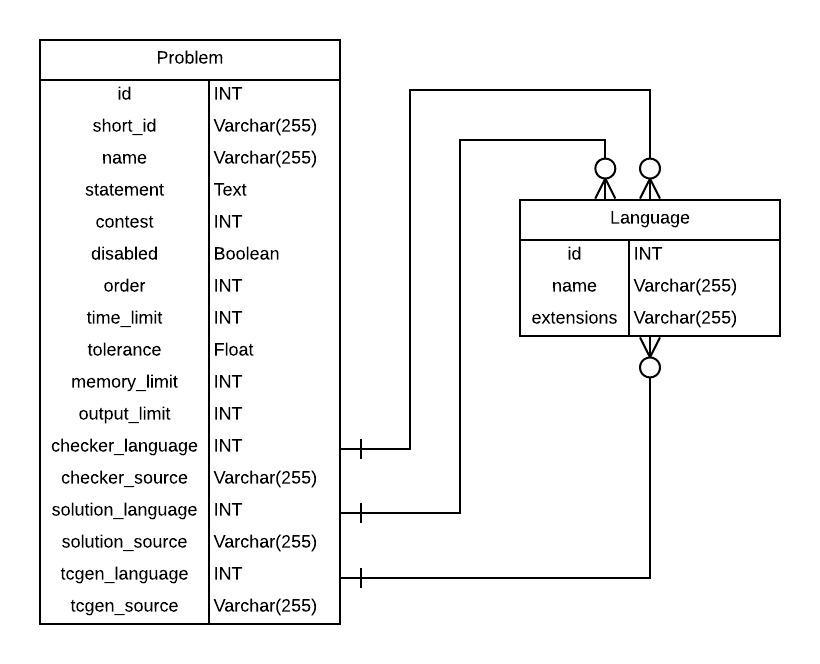
\includegraphics[width=0.8\textwidth]{images/problem-schema}
    \caption{Skema Basis Data Sistem Manajemen Soal}
    \label{fig:problem-schema}
\end{figure}

\par Setiap soal pada UGServer akan terikat pada suatu kompetisi. Suatu soal tidak dapat berada pada dua kompetisi sekaligus. Jika terdapat soal yang sama pada kompetisi yang berbeda, maka soal tersebut harus ditambahkan dua kali dan tetap dianggap soal yang berbeda. Setiap soal pada kompetisi memiliki nama dan \textit{short id}. Nama soal merupakan judul soal yang akan ditampilkan pada sistem antar muka yang digunakan pengguna. \textit{Short id} merupakan kode soal yang unik untuk setiap kompetisi dan mudah untuk dibaca oleh manusia. \textit{Short id} berguna untuk mengidentifikasi soal dengan mudah.

\par Informasi mengenai soal disimpan di sistem basis data pada tabel \textit{problems}. Skema basis data yang digunakan untuk menyimpan informasi soal digambarkan pada Gambar \ref{fig:problem-schema}. Aksi-aksi yang dapat dilakukan oleh pengguna terhadap soal ditentukan berdasarkan \textit{permission} yang dimiliki oleh pengguna tersebut.

% TODO: screenshot ui

\par Setiap soal memiliki deskripsi soal. Deskripsi soal merupakan penjelasan mengenai soal, format masukan, format keluaran, contoh masukan dan contoh keluaran. Deskripsi soal ditulis dalam format \textit{markdown} dan disimpan pada \textit{field} \textit{statement} pada tabel \textit{problems}. Pemilihan format \textit{markdown} bertujuan untuk kemudahan melakukan penyimpanan deskripsi soal. Beberapa sistem \textit{online judge} lain memungkinkan melakukan penyimpanan soal dalam bentuk \textit{file} seperti \textit{pdf}. UGServer tidak mendukung penyisipan \textit{file} pada deskripsi soal. Hal ini bertujuan untuk memudahkan implementasi.

\par Untuk melakukan penilaian terhadap jawaban peserta, setiap soal dilengkapi dengan beberapa informasi terkait penilaian. Beberapa informasi yang terkait dengan penilaian adalah: batas waktu eksekusi, batas penggunaan \textit{memory}, batas \textit{output file} yang dihasilkan, faktor toleransi, \textit{testcase generator}, solusi juri dan \textit{checker}. Batas waktu eksekusi disimpan pada \textit{field timelimit} dalam bentuk bilangan bulat yang menyatakan lamanya batas waktu eksekusi dalam satuan milidetik. Batas waktu ini digunakan oleh \textit{autograder} untuk menghentikan program secara paksa ketika berjalan terlalu lama. Batas penggunaan memory dan \textit{output file} yang dihasilkan disimpan pada \textit{field memorylimit} dan \textit{outputlimit} di tabel \textit{problems}. Batas tersebut disimpan dalam bentuk bilangan bulat yang menyatakan batas dalam satuan \textit{bytes}. Faktor toleransi disimpan pada \textit{field tolerance} di tabel \textit{problems} sebagai \textit{float}.

\par Dalam melakukan penilaian, \textit{autograder} memerlukan informasi mengenai \textit{testcase generator}, solusi juri, dan \textit{checker}. Informasi tersebut berupa \textit{source code} pada bahasa pemrograman tertentu. UGServer menyimpan informasi bahasa pemrograman yang digunakan oleh \textit{testcase generator}, solusi juri dan \textit{checker} pada sistem basis data sebagai \textit{foreign key} ke tabel \textit{languages}. Informasi bahasa pemrograman tersebut disimpan pada \textit{field tcgen\_language, solution\_language}, dan \textit{checker\_language} di tabel \textit{problems}. Informasi mengenai kode sumber tidak disimpan dalam sistem basis data karena dianggap kurang efisien jika ukuran \textit{source code} terlalu besar. Oleh karena itu, kode sumber disimpan sebagai \textit{file} yang berada pada \textit{disk}. Dengan begitu, sistem basis data hanya perlu menyimpan informasi mengenai alamat file dari \textit{source code} yang disimpan.

% TODO: graphql API

\par Pengguna dapat melakukan beberapa aksi pada soal yang ada pada sistem seperti: melihat daftar soal, membaca soal, menambah soal, mengubah soal, dan menghapus soal. Pengguna hanya dapat melakukan aksi-aksi tersebut sesuai izin yang dimilikinya seperti yang sudah dijelaskan pada bagian \ref{subsec:user-management}. Aksi-aksi tersebut dapat dilakukan menggunakan \textit{GraphQL API}.

\subsection{Manajemen Jawaban}

\par Peserta maupun juri dapat mengirimkan jawabannya terhadap suatu soal jika memiliki \textit{permission create:submissions}. Jawaban terhadap suatu soal berupa \textit{source code} yang ditulis pengguna dalam bahasa pemrograman tertentu yang diizinkan. Pada saat ini, bahasa pemrograman yang dapat digunakan adalah C dan C++. Pengguna dapat mengirimkan jawaban melalui \textit{GraphQL API}.

\begin{figure}[ht!]
    \centering
    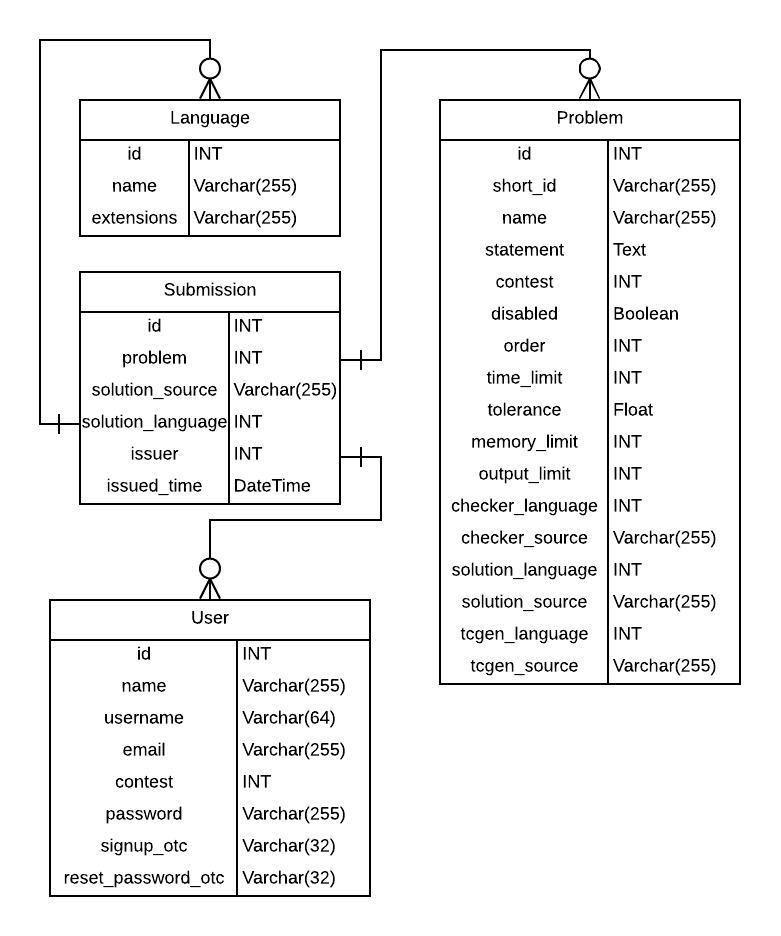
\includegraphics[width=0.8\textwidth]{images/submission-schema}
    \caption{Skema Basis Data Sistem Manajemen Jawaban}
    \label{fig:submission-schema}
\end{figure}

\par \textit{Source code} dari jawaban dari pengguna akan disimpan dalam bentuk \textit{file} yang berada pada \textit{disk}. Selain \textit{source code}, terdapat informasi lain pada jawaban pengguna yang disimpan seperti bahasa pemrograman yang digunakan, waktu pengiriman jawaban, pengirim jawaban dan soal yang bersangkutan. Informasi tersebut disimpan dalam basis data pada tabel \textit{submission}. Gambar \ref{fig:submission-schema} merupakan skema basis data yang digunakan untuk menyimpan jawaban.

\par Setiap jawaban yang berhasil dikirim oleh pengguna akan dinilai oleh \textit{grader}. \textit{Grader} akan berjalan secara otomatis ketika jawaban peserta disimpan. \textit{Grader} kemudian akan menentukan \textit{verdict} dari jawaban peserta. \textit{Verdict} merupakan hasil penilaian terhadap jawaban peserta. Jenis \textit{verdict} yang digunakan adalah:
\begin{enumerate}
    \item \textit{Accpeted}: menandakan bahwa jawaban memberikan keluaran yang benar dan memenuhi batasan.
    \item \textit{Wrong Answer}: menandakan bahwa jawaban memberikan keluaran yang salah tetapi memenuhi batasan.
    \item \textit{Memory Limit Exceeded}: menandakan bahwa jawaban menggunakan terlalu banyak \textit{memory} melebihi batasan yang ditetapkan.
    \item \textit{Time Limit Exceeded}: menandakan bahwa jawaban melebihi batasan waktu yang sudah ditetapkan.
    \item \textit{Runtime Error}: menandakan bahwa jawaban tidak berhasil dieksekusi karena adanya kesalahan pada jawaban.
    \item \textit{Compile Error}: menandakan jawaban tidak dapat dikompilasi.
    \item \textit{Internal Error}: menandakan adanya kesalahan pada sistem UGrade sehingga jawaban tidak dapat dinilai.
\end{enumerate}

\subsection{Penilain Jawaban}

\par Setiap jawaban yang dikirimkan oleh pengguna akan dinilai secara otomatis oleh UGServer. Penilaian dilakukan secara \textit{asynchronous}. Oleh karena itu, peserta tidak perlu menunggu penilaian selesai untuk melakukan aksi-aksi lain. Seringkali terdapat beberapa masalah teknis yang mengakibatkan jawaban peserta perlu dinilai ulang. Oleh sebab itu, setiap jawaban peserta dapat dinilai lebih dari satu kali. Hasil penilaian yang digunakan adalah hasil penilaian yang terakhir.

\subsubsection{\textit{Grading Group}}

\par Penilaian pada sebuah jawaban disebut sebagai \textit{grading group}. Setiap jawaban dapat dinilai lebih dari satu kali dan memiliki lebih dari satu \textit{grading group}. Adanya \textit{grading group} berguna untuk melakukan penilaian terhadap jawaban peserta lebih dari satu kali. Jika terdapat perubahan \textit{testcase} atau perubahan batasan waktu pada suatu soal, maka perlu adanya penilaian ulang. Penilaian ulang dapat dilakukan dengan membuat \textit{grading group} baru untuk setiap penilaian.

\begin{figure}[ht!]
    \centering
    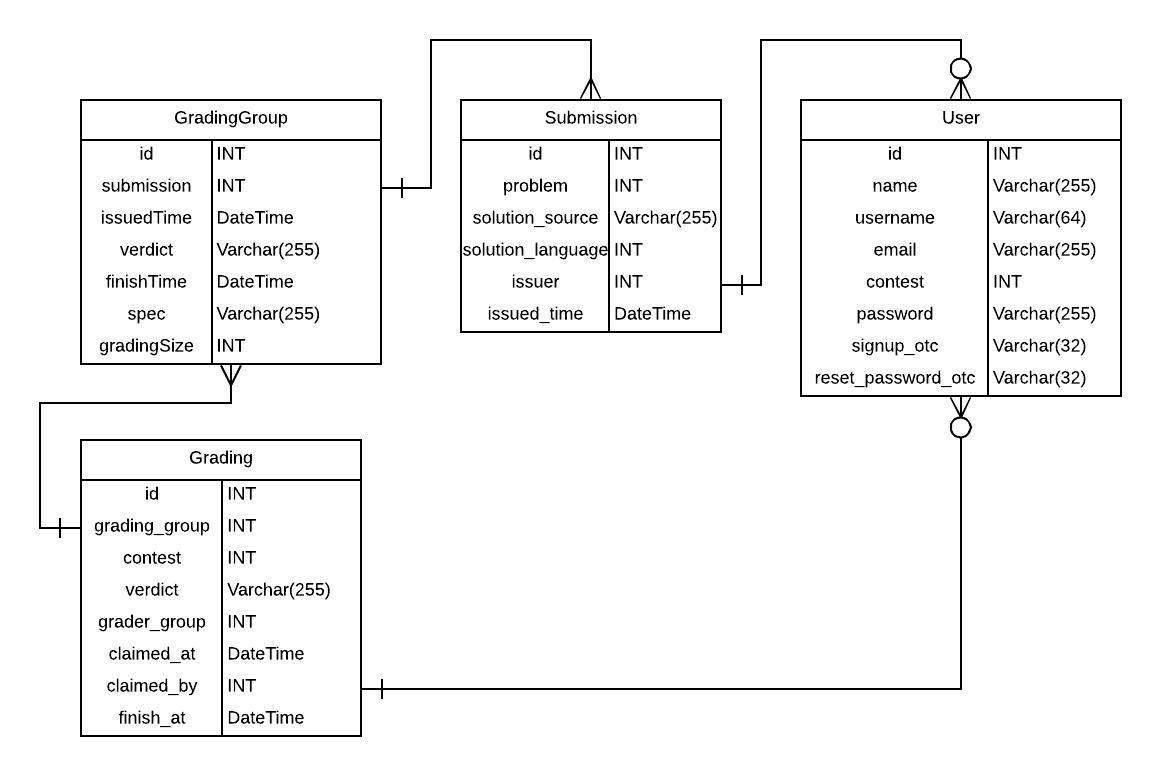
\includegraphics[width=\textwidth]{images/grader-schema}
    \caption{Skema Penilaian Jawaban Pengguna}
    \label{fig:grader-schema}
\end{figure}

\par Informasi dari \textit{grading group} disimpan dalam tabel \textit{GradingGroups} pada sistem basis data. Setiap \textit{grading group} memiliki informasi mengenai jawaban peserta, catatan waktu terciptanya \textit{grading group}, \textit{verdict}, spesifikasi penilaian, catatan waktu selesainya penilaian, dan \textit{grading size}. Informasi-informasi tersebut disimpan sebagai \textit{field} dalam tabel \textit{GradingGroups}. Spesifikasi penilaian berupa \textit{archive file} dan disimpan sebagai \textit{file} dalam \textit{disk}. Field \textit{spec} pada tabel \textit{GradingGroups} menyimpan informasi alamat \textit{file} dari spesifikasi penilaian. Skema basis data yang digunakan untuk melakukan penilaian ditunjukkan pada Gambar \ref{fig:grader-schema}.

\par Penilaian diawali dengan pembuatan spesifikasi penilaian. Spesifikasi penilaian berisi informasi mengenai \textit{testcase generator}, solusi juri, \textit{checker}, solusi peserta dan batasan soal. Informasi tersebut disimpan sebagai \textit{file} dengan format \textit{tar}. Spesifikasi penilain tersebut terdiri dari beberapa file sebagai berikut:
\begin{enumerate}
    \item tcgen.cpp\\ merupakan kode sumber \textit{testcase generator} dari soal. Ekstensi dari \textit{file} dapat berbeda sesuai bahasa pemrograman yang digunakan.
    \item solution.cpp\\ merupakan kode sumber  solusi juri pada soal yang bersangkutan. Ekstensi dari \textit{file} dapat berbeda sesuai bahasa pemrograman yang digunakan.
    \item checker.cpp\\ merupakan kode sumber \textit{checker} dari soal. Ekstensi dari \textit{file} dapat berbeda sesuai dengan bahasa pemrograman yang digunakan.
    \item submission.cpp\\ merupakan kode sumber solusi peserta. Ekstensi dari \textit{file} dapat berbeda sesuai dengan bahasa pemrograman yang digunakan.
    \item lang.json\\ \textit{file} ini berisi \textit{JSON document} yang menjelaskan bahasa pemrograman yang digunakan sebagai \textit{testcase generator}, solusi juri, \textit{checker} dan solusi peserta. \textit{JSON document} pada \textit{file} ini hanya berisi empat \textit{key} yaitu \textit{tcgen}, \textit{solution}, \textit{checker}, dan \textit{submission}. Setiap \textit{key} pada \textit{file} ini memiliki \textit{value} yaitu bahasa \textit{ID} dari bahasa pemrograman yang digunakan.
    \item problem.json\\ \textit{file} ini berisi \textit{JSON document} yang menjelaskan batasan dari soal. \textit{JSON document} pada file ini berisi empat buah \textit{key} yaitu \textit{timeLimit}, \textit{outputLimit}, \textit{memoryLimit}, dan \textit{tolerance}. Setiap \textit{key} pada \textit{file} ini memiliki \textit{value}  berupa bilangan yang menjelaskan batasan dari soal.
\end{enumerate}
\par \textit{File} spesifikasi penilaian ini nantinya akan diunduh oleh \textit{autograder} yang berjalan pada komputer pengguna.

\subsubsection{\textit{Grading Size}}

\par Setiap penilaian yang ditandai dengan \textit{grading group} memiliki suatu nilai \textit{grading size}. Nilai dari \textit{grading size} digunakan untuk mengurangi risiko serangan yang mungkin dilakukan pengguna. Sebuah penilaian dapat dilakukan oleh lebih dari satu \textit{worker}. Setiap worker akan memberikan hasil penilaiannya kepada UGServer. Jawaban peserta akan dinilai benar ketika mayoritas dari \textit{worker} yang melakukan penilaian memberikan \textit{verdict} \textit{accepted}. Nilai dari \textit{grading size} mengindikasikan banyaknya \textit{worker} yang melakukan penilaian.

\par Nilai \textit{grading size} yang besar akan lebih aman karena dapat lebih mengurangi risiko kecurangan peserta. Hal ini dikarenakan kemungkinan terjadinya kecurangan lebih kecil sebab \textit{worker} yang bekerja lebih banyak. Meskipun begitu, tingginya nilai \textit{grading size} menyebabkan proses penilaian menjadi lebih lambat karena penilaian harus menunggu banyak \textit{worker} untuk selesai terlebih dahulu. Sebaliknya, nilai \textit{grading size} yang kecil dapat mempercepat penilaian akan tetapi mengurangi keamanan. Nilai \textit{grading size} dapat diatur dalam pengaturan kompetisi oleh pengguna yang memiliki \textit{permission} \textit{update:contests}.

\par Karena setiap jawaban dapat dinilai lebih dari satu kali, perlu ada entitas yang merepresentasikan penilaian sebuah jawaban oleh sebuah \textit{worker}. Entitas tersebut dinamakan \textit{grading}. Sebuah \textit{grading} memiliki informasi mengenai \textit{grading group} terkait, \textit{verdict}, \textit{grader group}, catatan waktu penilaian, dan pengguna yang melakukan penilaian. Informasi ini disimpan di dalam basis data pada tabel \textit{Gradings}.

\par Secara singkat, setiap jawaban dapat memiliki beberapa \textit{grading group} yang merepresentasikan sebuah penilaian terhadap jawaban. Hasil penilaian jawaban pada sebuah \textit{grading group} merupakan hasil penilaian yang dilakukan oleh banyak \textit{worker}. Banyaknya \textit{worker} yang melakukan penilaian adalah sebanyak \textit{grading size}. Setiap penilaian yang dilakukan oleh \textit{worker} direpresentasikan menjadi sebuah \textit{grading}. Secara singkat dapat dikatakan bahwa setiap \textit{grading group} memiliki \textit{grading} sebanyak \textit{grading size}.

\subsubsection{\textit{Grader Group}}

\par Adanya nilai dari \textit{grading size} bertujuan agar setiap jawaban dapat dinilai lebih dari satu \textit{worker}. \textit{Worker} yang melakukan penilaian terhadap suatu jawaban tentunya harus merupakan \textit{worker} yang berbeda. Untuk mengatasi hal ini, setiap \textit{grading} dan \textit{worker} memiliki sebuah nilai \textit{grader group}. \textit{Worker} dengan nilai \textit{grader group} tertentu hanya dapat melakukan penialain terhadap \textit{grading} yang memiliki nilai \textit{grader group} yang sama. Setiap penilaian jawaban peserta, akan dibuat \textit{grading size} buah \textit{grading} yang memiliki nilai \textit{grader group} yang unik yaitu dari nol hingga $\textit{grading size} - 1$. Setiap \textit{worker} dengan \textit{grader group} $K$ hanya akan melakukan penilaian terhadap \textit{grading} yang memiliki nilai \textit{grader group} $K$.

\par Nilai \textit{grader group} dari setiap \textit{worker} dihitung dengan cara melakukan \textit{hash} pada ID \textit{worker}. Setiap \textit{worker} memiliki ID berupa integer yang unik. Nilai \textit{grader group} sebuah worker dihitung dengan formula $\textit{grader\_group} = hash(W_{id}) \bmod \textit{grading\_size}$. Dengan mengasumsikan jumlah \textit{worker} cukup banyak dibandingkan dengan nilai \textit{grading size}, maka cara ini akan mengelompokkan menjadi \textit{grading size} buah kelompok dengan anggota yang kira-kira sama banyak. Cara ini dipilih karena perhitungannya yang cepat, mudah dan dapat mengelompokkan \textit{worker} secara rata.

\begin{figure}[ht!]
    \centering
    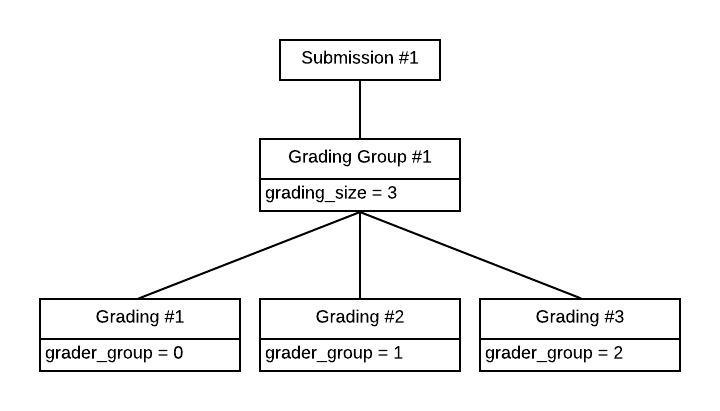
\includegraphics[width=0.6\textwidth]{images/grading-example-1}
    \caption{Contoh Proses Pembuatan \textit{Grading}}
    \label{fig:grading-example-1}
\end{figure}

\par Sebagai contoh, seorang pengguna telah melakukan pengiriman jawaban terhadap suatu soal. Setelah pengiriman jawaban tersebut berhasil dilakukan, akan tercipta sebuah \textit{submission} yang dapat kita beri nama \textit{Submission \#1}. UGServer kemudian akan secara otomatis membuat \textit{grading group} untuk menilai jawaban tersebut. Kita dapat memisalkan \textit{grading group} tersebut bernama \textit{Grading Group \#1}. Pada \textit{Grading Group \#1} terdapat informasi mengenai \textit{grading size}. Informasi \textit{grading size} didapatkan dari konfigurasi kompetisi. Pengguna dengan \textit{permission update:contest} dapat mengubah nilai ini. Dalam contoh ini, kita misalnya nilai \textit{grading size} dari kompetisi tersebut adalah tiga. Setelah \textit{grading group} terbentuk, UGServer akan membuat \textit{grading size} buah \textit{grading}. Dalam contoh ini berarti akan tercipta tiga buah \textit{grading}. Untuk kemudahan penjelasan, tiga buah \textit{grading} ini dapat kita sebut dengan \textit{Grading \#1} , \textit{Grading \#2}, dan \textit{Grading \#3}. Setiap \textit{grading} yang diciptakan akan memiliki nilai \textit{grader group} yang unik dan terurut dari nol hingga $\textit{grading size} - 1$. Dalam contoh ini \textit{Grading \#1} memiliki nilai \textit{grader group} nol, \textit{Grading \#2} memiliki nilai \textit{grader group} satu, dan \textit{Grading \#3} memiliki nilai \textit{grader group} dua. Gambar \ref{fig:grading-example-1} menggambarkan \textit{submission}, \textit{grading group} dan \textit{grading} pada contoh di paragraf ini.

\begin{figure}[ht!]
    \centering
    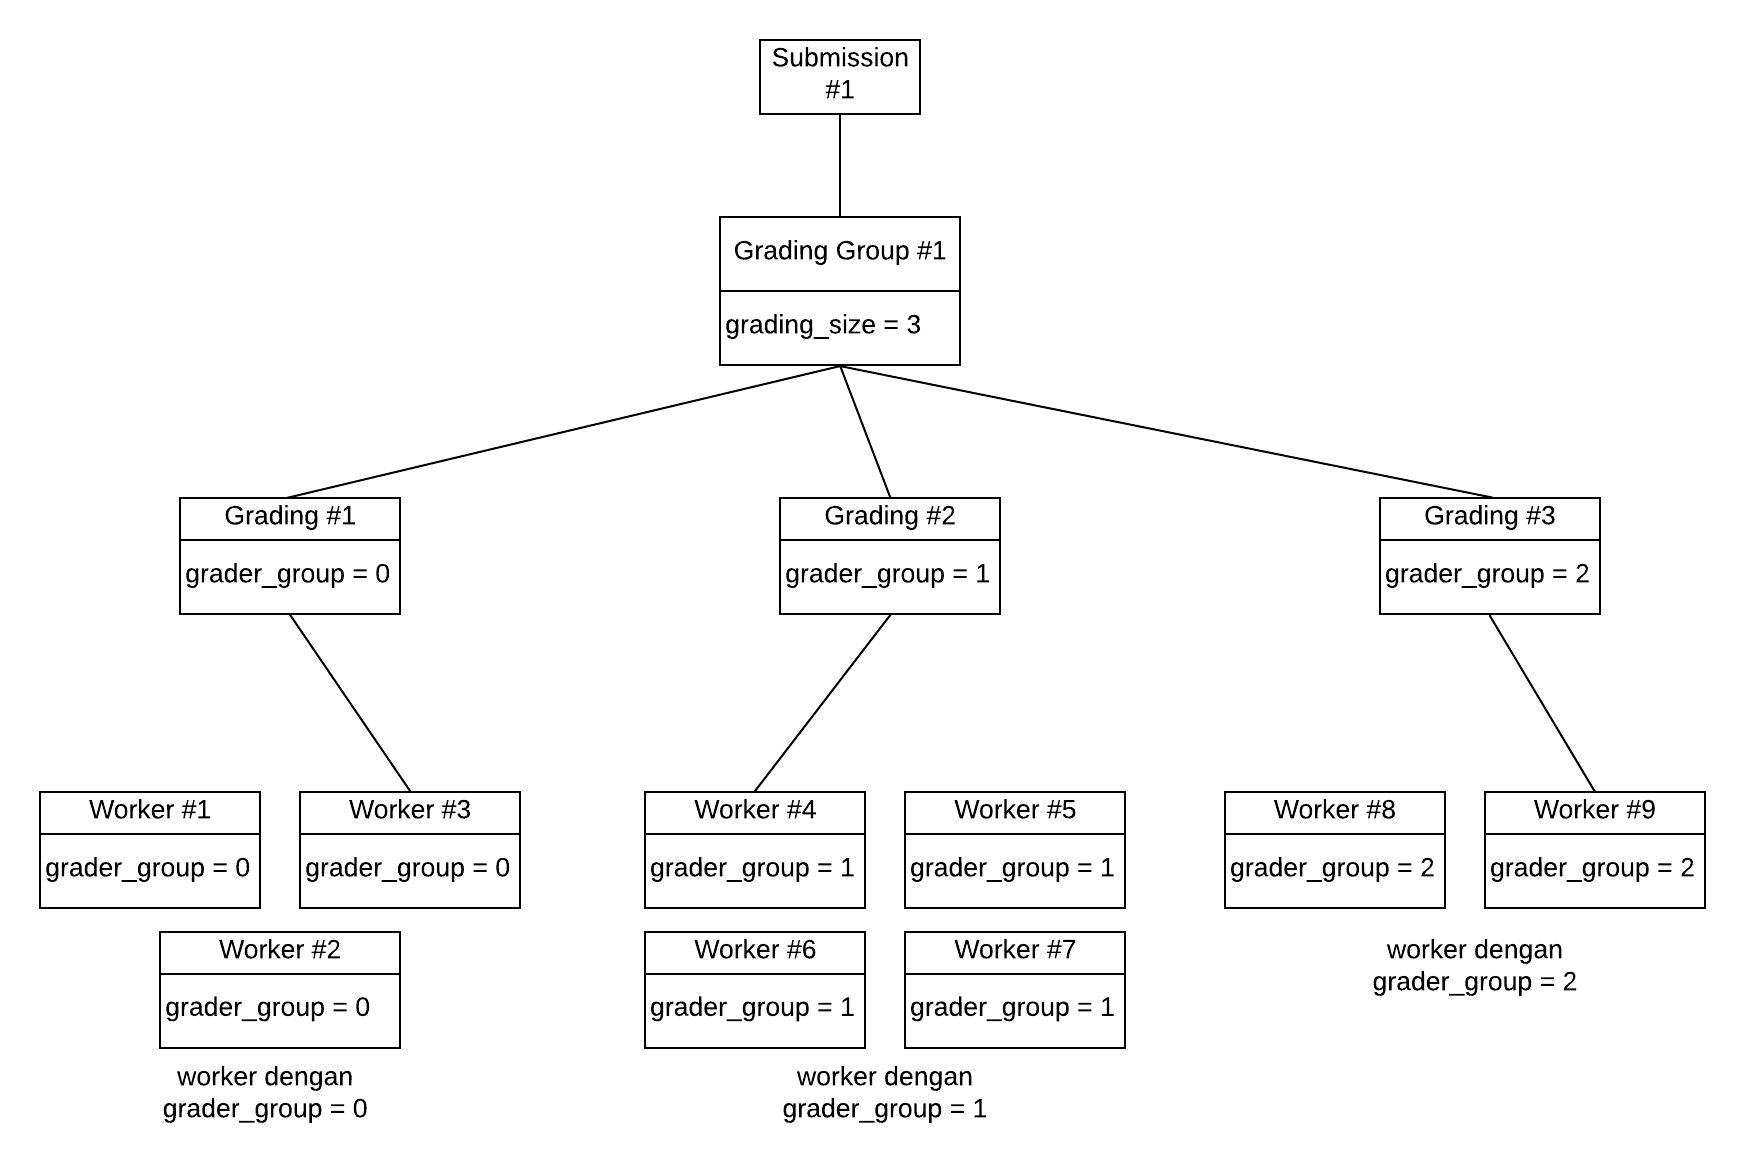
\includegraphics[width=\textwidth]{images/grading-example-2}
    \caption{Contoh Proses Penilaian Oleh \textit{Worker}}
    \label{fig:grading-example-2}
\end{figure}

\par Setelah terbentuk tiga buah \textit{grading} seperti pada paragraf sebelumnya, penilaian dapat mulai dilakukan oleh \textit{worker}. \textit{Worker} secara periodik akan selalu bertanya pada UGServer apakah terdapat \textit{grading} yang perlu dikerjakan. UGServer akan memberikan \textit{grading} yang sesuai dengan nilai dari \textit{grader group} \textit{worker} yang bersangkutan. Setiap \textit{grading} memiliki informasi \textit{claimed\_by} yang akan berisi ID dari peserta yang sedang melakukan penilaian terhadap \textit{grading} tersebut. Nilai tersebut bertujuan agar \textit{grading} yang sedang dinilai tidak akan dinilai oleh \textit{worker} lain. Gambar \ref{fig:grading-example-2} menjelaskan pemberian \textit{grading} pada \textit{worker} yang dilakukan oleh UGServer.

\par \textit{Worker} yang telah melakukan penilaian akan mengirimkan hasil penilaiannya kepada UGServer. UGServer kemudian akan mengubah nilai \textit{verdict} dari \textit{grading} dan mencatat waktu selesainya penilaian. Jika jumlah \textit{grading} yang selesai dinilai sudah lebih dari setengah dari \textit{grading size}, maka \textit{verdict} dari \textit{grading group} akan diubah. Setelah tahap tersebut, pengguna dapat melihat hasil akhir penilaiannya. 

% TODO: jelasin API waktu grading

% TODO: use more clear term for worker, grading group, grading size, grading, grader group.

% TODO: tambah kode assign grader group

% TODO: further works

\section{UGSbox}

% TODO: jelasin kodenya

\par Dalam menjalankan penilaian, UGSbox berperan dalam memberikan isolasi terhadap program-program yang berjalan di komputer pengguna. Program-program yang berjalan pada saat penilaian antara lain adalah: \textit{compiler}, \textit{testcase generator}, solusi peserta, solusi juri, dan \textit{checker}. Program-program ini dapat berisi kode yang membahayakan komputer pengguna yang menjalankannya. Oleh karena itu, diperlukan adanya sistem yang dapat mengisolasi program tersebut sehingga tidak membahayakan komputer pengguna. Pada tugas akhir ini, UGSbox berperan dalam memberikan isolasi tersebut.

\par UGSbox memberikan isolasi pada proses yang berjalan dengan menggunakan beberapa fitur dari linux. Isolasi yang diberikan \textit{ugsbox} antara lain adalah sebagai berikut:
\begin{itemize}
    \item isolasi \textit{filesystem}. \\ Isolasi terhadap \textit{filesystem} dilakukan dengan menggunakan \textit{system call chroot}. Dengan menggunakan \textit{chroot}, direktori \textit{root} dari suatu  proses dapat diganti menjadi direktori lain. Mengganti \textit{root} dari proses mengakibatkan proses tersebut tidak dapat mengakses \textit{file} yang ada di luar \textit{root}. \textit{Filesystem} yang akan digunakan oleh proses dapat dimuat dari \textit{file} yang memiliki format \textit{.tar.xz}. File tersebut dinamakan \textit{image file}. Proses isolasi \textit{filesystem} dimulai dengan melakukan ekstraksi \textit{image file} kemudian mengganti \textit{root} dari proses ke dalam direktori \textit{image file} yang sudah berhasil diekstrak. 

    \item \textit{filesystem binding}. \\ UGSbox memberikan fitur \textit{filesystem binding} yang dapat digunakan oleh pengguna untuk memasukkan \textit{filesystem} lain ke dalam \textit{filesystem} yang sudah diisolasi. Fitur ini berguna untuk menyimpan \textit{testcase} ke dalam suatu \textit{filesystem} khusus yang kemudian dapat dimuat ke dalam \textit{filesystem} yang sudah diisolasi.

    \item isolasi \textit{network}. \\ Untuk menjaga keamanan, setiap proses yang berjalan di dalam lingkungan yang diisolasi tidak boleh menggunakan \textit{network} untuk berkomunikasi dengan dunia luar. Untuk mengatasi masalah ini, UGSbox menggunakan fitur \textit{namespace} dari linux. Proses yang diisolasi akan mendapat \textit{namespace} dengan \textit{network interface} yang terisolasi dari \textit{network interface} milik \textit{host}.

    \item isolasi \textit{user}. \\ Selain isolasi \textit{network}, \textit{namespace} pada Linux juga digunakan untuk melakukan isolasi \textit{user}. Dengan mengisolasi \textit{user}, proses yang terisolasi tidak dapat mengetahui adanya \textit{user} lain di luar lingkungannya.

    \item batas penggunaan CPU dan \textit{memory}. \\ Penggunaan CPU dan \textit{memory} dari proses yang diisolasi tentunya perlu dibatasi. Hal ini bertujuan agar proses yang berjalan tidak memberatkan komputer pengguna ketika penilaian sedang berlangsung. Untuk mengatasi masalah ini, UGSbox menggunakan fitur \textit{cgroup} dari linux. Dengan menggunakan \textit{cgroup}, penggunaan \textit{memory} dan CPU dapat dibatasi dan dimonitor. Proses yang menggunakan CPU atau \textit{memory} melebihi batasan akan dihentikan secara paksa. 

    \item batas ukuran \textit{file} yang dapat dihasilkan. \\ Program yang dikirimkan oleh pengguna mungkin saja memuat kode yang dapat memberatkan \textit{disk} karena melakukan penulisan secara terus menerus. Hal ini dapat mengakibatkan komputer pengguna menjadi lambat karena \textit{disk}-nya tidak dapat digunakan. Untuk mengatasi masalah ini, UGSbox membatasi ukuran \textit{file} yang dapat diciptakan oleh proses di dalam lingkungan yang diisolasi. Pembatasan ini dicapai dengan menggunakan \textit{system call setrlimit}.

    \item batas jumlah \textit{file} yang dapat dibuka. \\ Untuk meningkatkan keamanan, jumlah \textit{file} yang dapat dibuka oleh proses yang diisolasi juga dibatasi menggunakan \textit{system call setrlimit}.

    \item batas proses yang dapat diciptakan. \\ Selain membatasi ukuran \textit{file} yang dihasilkan, dan jumlah \textit{file} yang dapat dibuka, UGSbox juga menggunakan \textit{setrlimit} untuk membatasi proses yang dapat diciptakan.

\end{itemize}

\begin{lstlisting}[caption={Contoh Hasil Eksekusi Perintah \textit{ugsbox}},label={lst:ugsbox-guard},language=Bash,style=BashStyle]
$ ugsbox guard --help
Usage:
  ugsbox guard [flags]

Flags:
  -b, --bind strings               bind host directory to sandbox directory with format <hostdir>:<sandboxdir>. Warning: file owner of binded directory will be changed
  -f, --file-size uint             generated file size limit
  -h, --help                       help for guard
  -i, --image string               compressed sandbox image (in .tar.xz) path
  -m, --memory-limit uint          memory limit in bytes (default 67108864)
  -M, --memory-throttle uint       memory throttle in bytes (default 268435456)
  -n, --nproc uint                 limit process creation e.g.: fork/exec
  -o, --open-file uint             open file limit
  -s, --stack-size uint            limit stack size in bytes
  -E, --stderr string              path (relative to sandbox) to file to be used as stderr
  -I, --stdin string               path (relative to sandbox) to file to be used as stdin
  -O, --stdout string              path (relative to sandbox) to file to be used as stdout
  -t, --time-limit uint            time limit in milisecond (default 10000)
  -T, --walltime-limit uint        wall clock time limit in milisecond (default 10000)
  -w, --working-directory string   working directory of process (default "/home")

Global Flags:
      --debug   show debug log
      --trace   show trace log
\end{lstlisting}

\par UGSBox dapat digunakan dengan dua cara yaitu: sebagai \textit{executable program} atau sebagai \textit{library}. Pengguna dapat menggunakan perintah \textit{ugsbox guard} untuk menjalankan UGSbox melalui CLI. Kode \ref{lst:ugsbox-guard} merupakan contoh hasil pemanggilan \textit{ugsbox guard}.

\par Selain melalui CLI, UGSbox juga dapat digunakan melalui pemanggilan fungsi pada bahasa pemrograman GO. Untuk dapat menggunakan UGSbox sebagai \textit{library}, pengguna dapat meng-\textit{import} \textit{package https://github.com/jauhararifin/ugrade} dan \textit{https://github.com/jauhararifin/ugrade/sandbox}. Penggunaan \textit{library} tersebut dapat dapat dilihat pada dokumentasi UGrade di \textit{https://godoc.org/github.com/jauhararifin/ugrade}.

\section{UGJob}

% TODO: jelasin kodenya

\par UGJob merupakan implementasi dari \textit{worker} pada keluarga perangkat lunak UGrade. UGJob dikembangkan menggunakan bahasa GO dan berperan dalam menilai jawaban pengguna. UGJob dikembangkan sebagai sebuah \textit{executable} yang dapat dijalankan melalui CLI. UGDesktop akan secara periodik menjalankan UGJob untuk melakukan penilaian.

\par Setiap \textit{grading} yang dihasilkan oleh UGServer akan dinilai oleh \textit{worker} yang ada pada komputer pengguna. \textit{Worker} pada komputer pengguna tidak perlu mengetahui adanya konsep \textit{grading group}, \textit{grading size}, dan \textit{grader group}. \textit{Worker} hanya perlu meminta \textit{grading} pada UGServer untuk dinilai. Dalam meminta \textit{grading}, \textit{worker} hanya perlu mengirimkan ID dari pengguna yang bertindak sebagai \textit{worker}. UGServer akan memberikan \textit{grading} yang sesuai dengan ID pengguna dari \textit{worker} tersebut.

\par Di sisi \textit{worker}, semua \textit{grading} yang perlu dinilai akan dipandang sebagai sebuah \textit{job}. Pada tugas akhir ini, \textit{job} dapat disamakan dengan \textit{grading} karena sebuah \textit{grading} akan dianggap sebagai sebuah \textit{job} oleh \textit{worker}. Istilah \textit{job} digunakan untuk meningkatkan abstraksi dari \textit{worker}. \textit{Worker} tidak perlu mengetahui konsep penilaian yang dilakukan di sisi UGServer. \textit{Worker} tidak perlu mengetahui adanya konsep \textit{grading} pada UGServer. Semua penilaian yang perlu dilakukan oleh \textit{worker} akan dianggap sebagai sebuah \textit{job}. Dengan menggunakan istilah \textit{job}, sistem penilaian yang ada pada sisi UGServer dapat dengan mudah dimodifikasi tanpa memengaruhi \textit{worker}.

\begin{lstlisting}[caption={Contoh Hasil Eksekusi Perintah \textit{ugjob consume}},label={lst:ugjob-consume},language=Bash,style=BashStyle]
$ ugjob consume --help
This program fetch job from server, execute it and send the result back to server.

Usage:
  ugjob consume [flags]

Flags:
  -h, --help                help for consume
  -u, --server-url string   Server url (default "http://localhost:8000")
  -t, --token string        Your session token

Global Flags:
      --debug   show debug message
      --trace   show trace message
\end{lstlisting}

\par UGJob dapat dijalankan melalui CLI dengan mengetikkan perintah \textit{ugjob consume}. UGJob memerlukan \textit{token} yang bisa didapatkan oleh pengguna pada saat melakukan \textit{sign in}. \textit{Token} ini berguna untuk mengidentifikasi ID dari pengguna. UGServer akan menggunakan \textit{token} untuk menentukan \textit{job} mana yang akan dikerjakan oleh \textit{worker}. Kode \ref{lst:ugjob-consume} merupakan contoh hasil pemanggilan \textit{ugjob consume}.

\par Pemanggilan \textit{ugjob consume} akan menjalankan \textit{worker} pada komputer pengguna dan proses penilaian akan mulai dilakukan. Penilaian diawali dengan pengambilan \textit{job} oleh UGJob. UGJob akan meminta \textit{job} kepada UGServer dengan mengirimkan \textit{GET HTTP request} ke UGServer dengan menyertakan \textit{token} yang dimilikinya. \textit{HTTP Request} tersebut akan dikirimkan ke URL \textit{/gradings} pada UGServer dengan menyertakan \textit{token} pada bagian \textit{header}.

\par Setiap permintaan \textit{job} yang dilakukan oleh UGJob akan diproses oleh UGServer. UGServer akan memberikan job yang sesuai kepada UGJob. Pemberian \textit{job} dilakukan dengan memandang \textit{token} yang disertakan oleh UGJob ketika melakukan permintaan \textit{job}. Jika tidak terdapat \textit{job} yang perlu dikerjakan, maka UGServer akan memberikan \textit{HTTP response} dengan status 404. UGServer akan memberikan \textit{job} kepada UGJob dengan bentuk \textit{tar file} yang dikirimkan melalui \textit{body} pada \textit{HTTP response}. Selain itu, UGServer juga menyertakan \textit{job token} pada setiap \textit{job} yang dikirimkan. \textit{Job token} ini berguna untuk membedakan antara satu buah \textit{job} dengan yang lainnya.

\par Setelah mendapatkan \textit{job} dari UGServer, UGJob akan melakukan penilaian dengan mengekstrak \textit{job} yang didapatkannya. \textit{Job} akan diekstrak pada suatu direktori sementara di \textit{/tmp}. Direktori \textit{/tmp} dipilih karena sistem secara otomatis akan menghapus isi dari direktori ini ketika \textit{booting}. Selain itu, direktori ini juga sudah standar digunakan sebagai tempat penyimpanan \textit{file} yang bersifat sementara. Direktori \textit{Job} yang sudah berhasil dinilai secara otomatis akan dihapus oleh UGJob. 

\subsection{Pembangkitan \textit{Testcase}}

\par Untuk melakukan penilaian, diperlukan adanya \textit{testcase}. \textit{Testcase} akan dibangkitkan dengan menggunakan program \textit{testcase generator} yang disertakan pada \textit{file} \textit{job}. \textit{Testcase generator} ini pertama-tama dikompilasi menjadi \textit{executable file} kemudian dijalankan. \textit{Testcase} yang dihasilkan oleh \textit{testcase generator} disimpan pada direktori sementara di dalam \textit{/tmp}.

% TODO: jelasin spesifikasi testcase generator & testcase suite

\par Program \textit{testcase generator} hanya membangkitkan masukan dari \textit{testcase}. Keluaran dari \textit{testcase} dibangkitkan dengan menggunakan solusi juri. Untuk membangkitkan keluaran dari \textit{testcase}, solusi juri dikompilasi kemudian dijalankan dengan memberikan input yang berasal dari \textit{testcase generator}. Keluaran dari solusi juri ini akan digunakan sebagai keluaran dari \textit{testcase}.

\par \textit{Testcase} yang sudah terbentuk disimpan pada suatu direktori tertentu. Direktori yang menjadi tempat penyimpanan \textit{testcase} tidak akan dihapus ketika penilaian sudah selesai dilakukan. Hal ini bertujuan agar proses penilaian \textit{job} selanjutnya tidak perlu melakukan pembangkitan \textit{testcase} lagi.

\subsection{Penghitungan Waktu Dan \textit{Memory} Solusi Juri} 

\par Waktu dan \textit{memory} dari eksekusi solusi juri perlu dihitung untuk menentukan batasan waktu dan \textit{memory} solusi peserta. Waktu dan \textit{memory} eksekusi solusi juri dihitung pada saat pembangkitan \textit{testcase}. Solusi juri diperlukan dalam membangkitkan keluaran dari \textit{testcase}. Pada saat keluaran \textit{testcase} dibangkitkan, lamanya waktu eksekusi dan penggunaan \textit{memory}-nya dihitung dan dicatat.

\par Perhitungan waktu eksekusi dilakukan dengan menggunakan UGSbox. Proses yang dijalankan menggunakan UGSbox dapat dihitung penggunaan waktu dan \textit{memory}-nya. Jika solusi juri melebihi batas waktu yang ditentukan oleh juri, maka UGJob akan memberikan \textit{verdict} \textit{internal error} yang menandakan bahwa penilaian gagal dilakukan. Hal ini dapat terjadi ketika komputer peserta sangat lambat.

\subsection{Eksekusi Solusi Peserta}

\par Setelah \textit{testcase} berhasil dibangkitkan dan batasan untuk peserta sudah berhasil dihitung, solusi peserta akan mulai dijalankan. Seperti program lainnya, solusi peserta dijalankan menggunakan UGSbox untuk menghindari penggunaan \textit{resource} yang berlebihan dan menghindari risiko dari adanya serangan yang ada pada program solusi peserta.

\par Sebelum solusi peserta dijalankan, tentunya perlu ada proses kompilasi. Proses kompilasi ini dilakukan dengan cara yang sama untuk mengkompilasi program lain. Pada saat kompilasi, beberapa kegagalan mungkin terjadi seperti: kesalahan \textit{syntax}, penggunaan \textit{memory} terlalu besar, dan proses kompilasi berjalan terlalu lama. Jika terjadi kegagalan pada tahap kompilasi, maka UGJob akan memberikan \textit{verdict} \textit{compile error}.

\par Penggunaan CPU dan \textit{memory} dari program solusi peserta dibatasi berdasarkan batasan yang diperoleh ketika menjalankan program solusi juri. Jika solusi peserta menggunakan \textit{memory} melebihi batasan yang sudah dihitung, maka UGJob akan memberikan \textit{verdict} \textit{memory limit exceeded}. Selain itu, jika solusi peserta berjalan terlalu lama dan melebihi batasan waktu yang sudah dihitung maka UGJob akan memberikan \textit{verdict} \textit{time limit exceeded}. Program solusi peserta mungkin saja melakukan kesalahan yang menyebabkan munculnya \textit{error} seperti pembagian dengan nol, atau mengakses alamat \textit{memory} yang belum dialokasikan. Jika hal ini terjadi, maka UGJob akan memberikan \textit{verdict} \textit{runtime error}.

\par Keluaran dari program solusi peserta disimpan pada direktori sementara yang diletakkan pada \textit{/tmp}. Selanjutnya keluaran dari program solusi peserta akan dinilai dengan cara dibandingkan dengan keluaran solusi juri. Setelah penilaian selesai dilakukan, keluaran program solusi peserta sudah tidak digunakan lagi. Oleh sebab itu, keluaran program solusi peserta dihapus setelah penilaian selesai dilakukan.

\subsection{Penilaian Keluaran Solusi Peserta}

\par Keluaran dari program solusi peserta perlu dinilai kebenarannya. Penilaian kebenaran dari program solusi peserta dilakukan dengan cara membandingkannya dengan keluaran solusi juri. UGJob membandingkan keluaran program solusi peserta dengan program solusi juri dengan menggunakan \textit{checker}.

\par \textit{Checker} merupakan sebuah program yang dibuat oleh juri dan digunakan untuk menilai kebenaran program solusi peserta. Seperti pada program lainnya, perlu adanya proses kompilasi yang dilakukan pada \textit{checker}. Proses kompilasi \textit{checker} dilakukan dengan cara yang sama seperti kompilasi program lainnya.

\lstinputlisting[caption={Contoh Program \textit{Checker}},label={lst:exact-match-checker},language=C,style=CStyle]{listings/exact-match-checker.c}

\par Setelah \textit{checker} selesai dikompilasi, \textit{checker} akan dijalankan dengan memberikan masukan berupa masukan \textit{testcase}, keluaran program solusi juri dan keluaran program solusi peserta. \textit{Checker} kemudian akan memberikan keluaran berupa kebenaran dari program solusi peserta. Kode \ref{lst:exact-match-checker} merupakan contoh \textit{checker} yang membandingkan kesamaan tiap \textit{byte} dari keluaran solusi peserta dan solusi juri.

\par Program \textit{checker} akan memberikan keluaran berupa \textit{string} yang dapat bernilai \textit{AC} atau \textit{WA}. Keluaran \textit{checker} akan bernilai \textit{AC} jika solusi peserta dianggap benar, dan akan bernilai \textit{WA} jika sebaliknya. UGJob kemudian akan mengirimkan \textit{verdict} kepada UGServer sesuai dengan hasil penilaian \textit{checker}.

\par Program \textit{checker} yang dibuat oleh juri mungkin saja memiliki kesalahan. Kesalahan tersebut mengakibatkan program \textit{checker} menghasilkan \textit{error}. Selain itu, jika program \textit{checker} juga mungkin menggunakan terlalu banyak \textit{memory} dan menghabiskan terlalu banyak \textit{waktu}. Jika hal ini terjadi, maka program \textit{checker} akan dihentikan dan UGJob akan menghasilkan \textit{verdict} \textit{internal error}.

\par Setelah penilaian selesai dilakukan dan \textit{verdict} sudah ditentukan, hasil penilaian akan dikirmkan ke UGServer. Hasil penilaian yang dikirimkan berupa \textit{verdict} hasil penilaian. Pengiriman dilakukan melalui \textit{POST HTTP request}. \textit{Job token} disertakan pada \textit{header} dari \textit{HTTP request} sebagai identitas dari \textit{job} yang telah diselesaikan.

\section{UGDesktop}

\par Dalam kelompok perangkat lunak UGrade, pengguna dapat berinteraksi dengan sistem kompetisi dengan UGDesktop. UGDesktop memudahkan interaksi pengguna dengan memberikan antar-muka berbasis grafis. Pengguna dapat meng-\textit{install} UGDesktop pada komputernya. Pengguna kemudian dapat menjalankan UGDesktop sebagai aplikasi \textit{desktop} pada komputernya.

\begin{figure}[ht!]
    \centering
    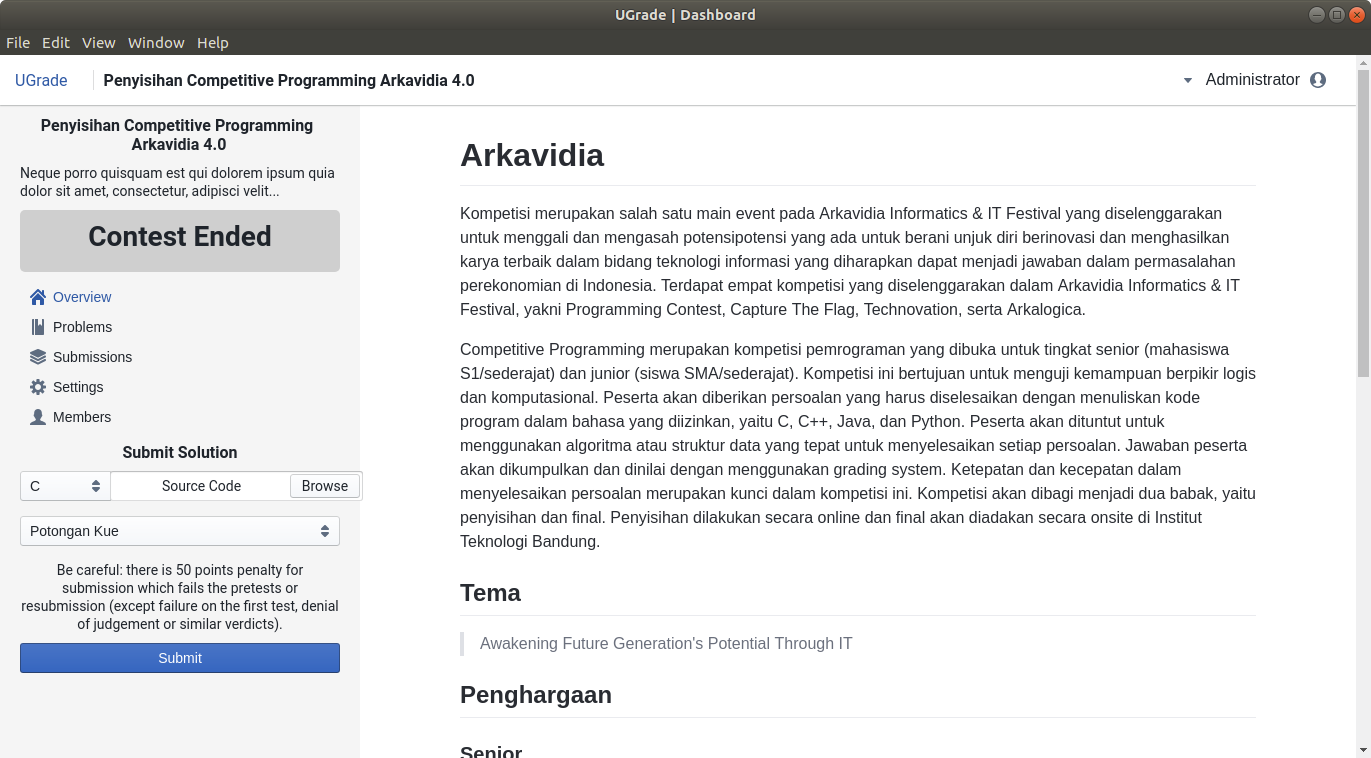
\includegraphics[width=\textwidth]{images/ugdesktop-example}
    \caption{Halaman Kompetisi Dari UGDesktop}
    \label{fig:ugdesktop-example}
\end{figure}

\par UGDesktop dikembangkan menggunakan \textit{typescript}, \textit{react} dan \textit{electron}. \textit{React} dipilih karena mudah untuk digunakan dan banyak \textit{library} yang mendukung pengembangan aplikasi berbasis \textit{react}. \textit{React} umumnya digunakan untuk mengembangkan aplikasi berbasis \textit{web} dan membutuhkan \textit{web browser} untuk menjalankan aplikasi tersebut. Pengguna membutuhkan aplikasi yang dapat berjalan sebagai \textit{desktop app} untuk dapat menjalankan sistem antar muka pengguna sekaligus \textit{worker}. Untuk mengatasi hal tersebut, \textit{electron} digunakan untuk menjalankan aplikasi \textit{web} yang berbasis \textit{react} sebagai aplikasi \textit{desktop}. Gambar \ref{fig:ugdesktop-example} merupakan contoh salah satu halaman pada UGDesktop.

\par Untuk melakukan penilaian, UGDesktop secara periodik akan meminta menjalankan UGJob. Dalam menjalankan UGJob, UGDesktop menggunakan \textit{token} yang didapatkannya ketika pengguna melakukan \textit{sign in}. UGJob yang dijalankan UGDesktop akan meminta \textit{job} dari UGServer untuk dinilai.

\section{Pengujian}

\par Pada tugas akhir ini, dilakukan tiga pengujian terhadap yaitu kinerja, kebenaran dan keamanan. Kinerja dari sistem yang dibangun pada tugas akhir ini diuji dengan melakukan simulasi pengiriman jawaban oleh peserta. Untuk mengukur peningkatan kinerja, sistem \textit{online judge} yang dibangun dibandingkan dengan sistem \textit{online judge} lain yang populer digunakan untuk menyelenggarakan kompetisi \textit{competitive programming}. Kebenaran dari sistem yang dibangun diuji dengan mengirimkan berbagai jenis jawaban kepada sistem. Kebenaran dari sistem ditentukan berdasarkan hasil yang diberikan oleh sistem terhadap berbagai jenis jawaban yang dinilai. Keamanan dari sistem diuji dengan melakukan beberapa jenis serangan kepada sistem. Keamanan dari sisem ditentukan berdasarkan ketahanan sistem terhadap serangan-serangan yang diberikan.

\subsection{Pengujian Kinerja}

\par Pengujian kinerja dilakukan dengan menyimulasikan proses pengiriman jawaban oleh pengguna. Sebuah kompetisi diciptakan dengan beberapa pengguna yang akan mengirimkan jawaban secara periodik. Kinerja sistem yang dibangun dibandingkan dengan sistem \textit{online judge} yang bersifat \textit{open source} yaitu DOMJudge. DOMJudge dipilih karena bersifat \textit{open source} dan sudah populer digunakan untuk menyelenggarakan kompetisi \textit{competitive programming}. DOMJudge telah digunakan untuk menyelenggarakan ACM-ICPC, Arkavidia, Vocompfest dan banyak kompetisi lainnya.

\par Lima belas peserta disiapkan untuk melakukan pengujian kinerja sistem \textit{online judge} yang akan dibandingkan. Lima belas peserta tersebut akan mengirimkan beberapa \textit{source code} kepada sistem \textit{online judge} secara periodik. Pengujian dilakukan dengan membuat sebuah soal \textit{competitive programming}. Soal yang digunakan pada pengujian adalah soal perkalian dua buah polinomial berderajat $N$. Kompleksitas yang diharapkan oleh juri dari soal tersebut adalah $O(N log N)$. Soal ini dipilih karena memiliki beragam solusi dengan kompleksitas yang berbeda-beda. Solusi dengan kompleksitas yang lebih buruk dari $O(N log N)$ akan dianggap sebagai solusi yang salah.

\begin{figure}[ht!]
    \centering
    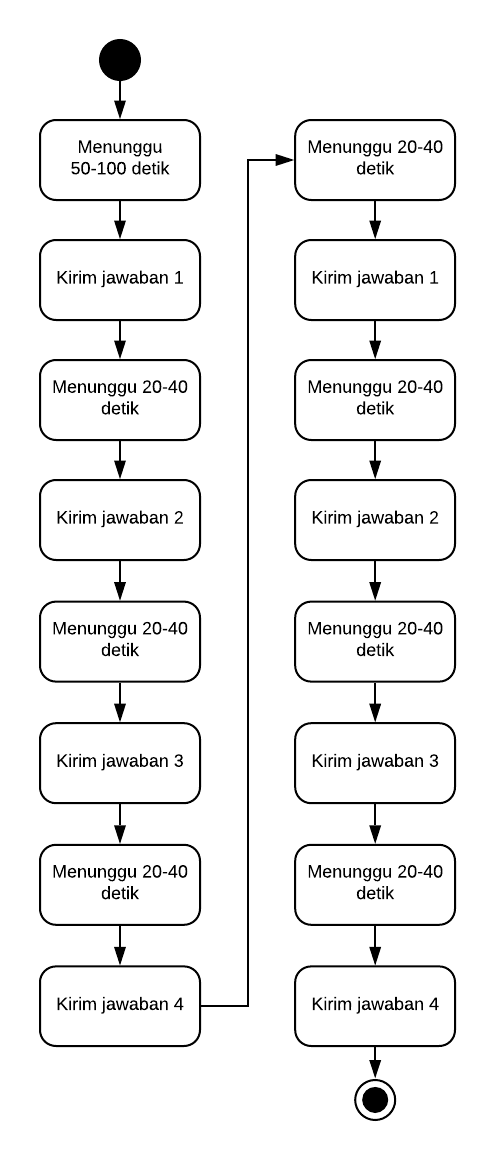
\includegraphics[width=0.5\textwidth]{images/performance-testing-activity}
    \caption{Diagram Aktivitas Dari Pengiriman Jawaban Peserta}
    \label{fig:performance-testing-activity}
\end{figure}

\par Setiap peserta dari lima belas peserta yang telah disiapkan akan menunggu selama lima puluh hingga seratus detik kemudian mengirimkan jawaban secara periodik tiap dua puluh hingga empat puluh detik. Terdapat empat jenis jawaban yang akan dikirimkan oleh peserta yaitu:
\begin{enumerate}
    \item Jawaban dengan kompleksitas $O(N log N)$. Jawaban ini merupakan jawaban yang diharapkan oleh juri dan akan dinilai sebagai jawaban yang benar.
    \item Jawaban dengan kompleksitas $O(N^{log_2{3}})$.
    \item Jawaban dengan kompleksitas $O(N^2)$.
    \item Jawaban dengan kompleksitas $O(N^2)$ tetapi berbeda implementasi dengan jawaban ketiga.
\end{enumerate}
Setiap peserta akan mengirimkan empat jawaban tersebut secara periodik. Setiap jawaban dari empat jawaban tersebut akan dikirimkan oleh setiap peserta sebanyak dua kali. Jumlah jawaban yang dikirimkan oleh peserta adalah delapan buah jawaban karena setiap peserta mengirimkan setiap jenis jawaban dua kali. Setelah delapan buah jawaban tersebut dikirimkan oleh peserta, peserta akan berhenti mengirimkan jawaban. Diagram aktivitas pada Gambar \ref{fig:performance-testing-activity} menggambarkan alur pengiriman jawaban yang dilakukan oleh setiap peserta.

\par Sistem \textit{online judge} yang akan diuji (DOMJudge dan UGrade) di-\textit{deploy} dengan menggunakan layanan EC2 (\textit{elastic compute cloud}) dari AWS (Amazon Web Service). DOMJudge terdiri dari dua jenis program yaitu DOMServer dan JudgeHost. DOMServer merupakan program yang digunakan oleh DOMJudge sebagai sistem manajemen kompetisi sedangkan JudgeHost merupakan program yang berperan sebagai \textit{autograder}. Pada pengujian kinerja, DOMServer dijalankan pada mesin EC2 dengan tipe \textit{t2.medium}. Mesin tersebut memiliki RAM sebesar 4GB dan dua buah \textit{virtual} CPU. Jenis mesin ini dipilih karena murah dan cukup untuk menangani pengiriman jawaban dari pengguna. JudgeHost dijalankan pada EC2 dengan tipe \textit{t2.micro} yang memiliki 1GB RAM dan satu buah \textit{virtual} CPU. EC2 jenis tersebut dipilih karena murah dan cukup untuk melakukan penilaian jawaban peserta.

\par DOMJudge diuji dengan menjalankan satu buah DOMServer dan dua buah JudgeHost. JudgeHost dijalankan pada dua buah mesin karena umumnya dua buah mesin sudah lebih dari cukup untuk melakukan penilaian jawaban lima belas peserta. Keputusan ini didasari oleh keberjalanan kompetisi \textit{competitive programming} Arkavidia pada tahun 2018 yang diikuti lebih dari seratus orang dengan hanya menggunakan enam buah JudgeHost. Kompetisi tersebut berjalan dengan lancar sehingga dua buah JudgeHost dinilai cukup untuk menilai jawaban dari lima belas orang peserta.

\par Pengujian pada sistem \textit{online judge} dilakukan sebanyak tiga kali. Hal ini bertujuan untuk meningkatkan keakuratan pengujian. Waktu lamanya penilaian sebuah jawaban dan banyaknya antrian jawaban yang ada pada sistem dicatat untuk menentukan kinerja sistem. Tabel \ref{tab:domjudge-wait-time}, \ref{tab:domjudge-process-time} dan \ref{tab:domjudge-system-time} memaparkan data hasil pengujian kinerja sistem \textit{online judge} DOMJudge. Gambar \ref{fig:domjudge-queue} manggambarkan jumlah jawaban yang berada pada antrian sistem DOMJudge dari waktu ke waktu. Terdapat tiga jenis besaran yang dihitung untuk menentukan kinerja DOMJudge yaitu:
\begin{enumerate}
  \item Waktu tunggu \\ Waktu tunggu didefinisikan sebagai lamanya sebuah jawaban berada pada antrian sistem. Jawaban berada pada antrian sistem mulai dari jawaban tersebut dikirim hingga jawaban tersebut mulai dinilai oleh \textit{autograder}.
  \item Waktu pemrosesan \\ Waktu pemrosesan didefinisikan sebagai lamanya sebuah jawaban dinilai oleh \textit{autograder}. Sebuah jawaban mulai dinilai ketika \textit{worker} dari \textit{autograder} mengambil jawaban tersebut dari antrian sistem.
  \item Waktu penilaian \\ Waktu penilaian didefinisikan sebagai lamanya sebuah jawaban mulai dikirim hingga selesai dinilai. Secara sederhana waktu penilaian merupakan total lamanya sebuah jawaban berada dalam sistem \textit{online judge}. Waktu penilaian juga dapat dipandang sebagai total dari waktu tunggu, waktu pemrosesan dan waktu pengiriman jawaban. Untuk melakukan penilaian, \textit{worker} perlu mengambil jawaban yang ada pada antrian sistem \textit{online judge}. Pengambilan jawaban dari antrian sistem memerlukan waktu karena jawaban perlu dikirimkan melalui jaringan sehingga menimbulkan adanya tambahan waktu yang berupa \textit{network latency}. Pada pengujian yang dilakukan, nilai dari \textit{network latency} sangat kecil dan dapat diabaikan. Karena kecilnya \textit{network latency}, waktu penilaian dapat dipandang sebagai total dari waktu tunggu dan waktu pemrosesan.
\end{enumerate}

\begin{table}[ht]
    \centering
    \begin{tabular}{| c | c | c | c |}
    \hline
    Nomor pengujian & Minimum (detik) & Maksimum (detik) & Rata-rata (detik) \\
    \hline
    \hline
    1 & 0.068 & 384.008 & 188.073 \\
    \hline
    2 & 0.143 & 384.832 & 192.339 \\
    \hline
    3 & 1.3138 & 390.6347 & 194.1095 \\
    \hline
\end{tabular}
    \caption{Data Waktu Tunggu Pada Pengujian Kinerja DOMJudge.}
    \label{tab:domjudge-wait-time}
\end{table}

\begin{table}[ht]
    \centering
    \begin{tabular}{| c | c | c | c |}
    \hline
    Nomor pengujian & Minimum (detik) & Maksimum (detik) & Rata-rata (detik) \\
    \hline
    \hline
    1 & 9.0931 & 12.4293 & 10.011825 \\
    \hline
    2 & 9.0994 & 16.1991 & 10.06895833 \\
    \hline
    3 & 9.0742 & 15.9872 & 10.05397167 \\
    \hline
\end{tabular}
    \caption{Data Waktu Pemrosesan Pada Pengujian Kinerja DOMJudge.}
    \label{tab:domjudge-process-time}
\end{table}

\begin{table}[ht]
    \centering
    \begin{tabular}{| c | c | c | c |}
    \hline
    Nomor pengujian & Minimum (detik) & Maksimum (detik) & Rata-rata (detik) \\
    \hline
    \hline
    1 & 12.3457 & 393.2282 & 198.0845733 \\
    \hline
    2 & 16.3426 & 393.9705 & 202.4083175 \\
    \hline
    3 & 17.301 & 399.7231 & 204.1634717 \\
    \hline
\end{tabular}
    \caption{Data Waktu Penilaian Pada Pengujian Kinerja DOMJudge.}
    \label{tab:domjudge-system-time}
\end{table}

\par Berdasarkan Tabel \ref{tab:domjudge-system-time}, dapat dikatakan bahwa waktu penilaian dari DOMJudge berkisar antara lima belas detik hingga empat ratus detik dengan rata-rata sekitar dua ratus detik. Berdasarkan data tersebut, dapat dikatakan bahwa setiap peserta rata-rata perlu menunggu sekitar tiga hingga empat menit untuk mengetahui nilai dari jawaban yang dikirimkannya. Waktu penilaian ini tergolong tinggi untuk penilaian yang dilakukan oleh \textit{autograder}. Menurut \cite{danutamalms}, waktu penilaian yang dilakukan oleh \textit{autograder} bernilai kurang lebih sepuluh detik. 

\par Waktu penilaian yang tinggi pada pengujian kinerja DOMJudge disebabkan oleh jumlah \textit{worker} yang tidak sebanding dengan jumlah jawaban yang dikirimkan oleh peserta. Umumnya, pada kompetisi \textit{competitive programming}, peserta jarang melakukan pengiriman jawaban dalam rentang waktu yang singkat, akan tetapi pengujian dilakukan dengan cara menyimulasikan peserta untuk mengirimkan jawaban dalam waktu yang singkat. Hal tersebut bertujuan untuk merepresentasikan keadaan dimana peserta kompetisi berjumlah banyak dan jawaban yang harus dinilai oleh sistem berjumlah banyak dalam waktu yang singkat. Sebenarnya pengujian dapat dilakukan dengan cara meningkatkan jumlah peserta, akan tetapi cara tersebut tidak digunakan karena membutuhkan biaya yang besar. Oleh karena itu, pengujian pada tugas akhir ini dilakukan dengan lima belas peserta yang melakukan pengiriman jawaban dalam waktu yang singkat (dua puluh hingga empat puluh detik).

\begin{figure}[ht!]
    \centering
    \begin{tikzpicture}
    \begin{axis}[xlabel={Waktu (detik)}, ylabel={Jumlah jawaban pada antrian}, xmin=0,xmax=700, ymin=0, ymax=100, legend pos=north east, ymajorgrids=true, grid style=dashed,]
        \addplot[color=blue,] table {data/domjudge-queue-test1.txt};
        \addlegendentry{Pengujian pertama}
        \addplot[color=red,] table {data/domjudge-queue-test2.txt};
        \addlegendentry{Pengujian kedua}
        \addplot[color=green] table {data/domjudge-queue-test3.txt};
        \addlegendentry{Pengujian ketiga}
    \end{axis}
\end{tikzpicture}
    \caption{Diagram Jumlah Jawaban Pada Antrian DOMJudge.}
    \label{fig:domjudge-queue}
\end{figure}

% jelasin gambar fig:domjudge-queue
\par Gambar \ref{fig:domjudge-queue} merupakan grafik yang memaparkan jumlah antrian pada DOMJudge seiring berjalannya waktu. Berdasarkan gambar tersebut, puncak jumlah antrian jawaban dari sistem DOMJudge memiliki nilai yang cukup tinggi yaitu tujuh puluh buah jawaban. Dari gambar tersebut terlihat bahwa jumlah antrian pada DOMJudge terus meningkat hingga mencapai suatu puncak tertentu kemudian menurun hingga mencapai angka nol. Terjadinya peningkatan jumlah antrian di awal waktu tersebut disebabkan karena peserta sedang aktif mengirimkan jawaban kepada sistem sedangkan seluruh \textit{worker} sedang sibuk melakukan penilaian. Karena tidak ada \textit{worker} yang tersedia, jawaban peserta terus menerus dimasukkan kedalam antrian sistem dan mengakibatkan jumlah antrian sistem terus meningkat. Tidak tersedianya \textit{worker} tersebut disebabkan karena jumlah \textit{worker} yang tidak sebanding dengan jumlah peserta. Setelah jumlah antrian sistem mencapai puncaknya, jumlah antrian tersebut perlahan-lahan mulai turun. Hal ini disebabkan karena peserta sudah tidak aktif mengirimkan jawaban sehingga jumah antrian tidak bertambah lagi dan mulai turun karena \textit{worker} masih melakukan penilaian pada sisa jawaban di antrian tersebut.  

\par Sistem \textit{online judge} yang dibangun pada tugas akhir ini (UGrade) diuji dengan cara yang sama seperti DOMJudge. Seperti DOMJudge, UGrade juga memiliki dua jenis program yang harus dijalankan yaitu sistem manajemen kompetisi dan \textit{autograder}. Pada UGrade, program yang menjadi sistem manajemen kompetisi adalah UGServer dan program yang menjadi \textit{autograder} adalah UGJob. Pengujian dilakukan dengan menyimulasikan pengiriman jawaban oleh lima belas peserta seperti yang dilakukan pada pengujian DOMJudge.

\par Seperti pada pengujian DOMJudge, sistem manajemen kompetisi UGrade (UGServer) dijalankan pada mesin EC2 yang bertipe \textit{t2.medium}. Karena pada UGrade setiap peserta bertindak sebagai \textit{autograder}, maka pada pengujian ini setiap peserta diberikan sebuah mesin sendiri. Mesin yang digunakan untuk menjalankan \textit{autograder} ini merupakan mesin EC2 yang bertipe \textit{t2.micro}. Mesin tersebut dipilih untuk menyamakan lingkungan \textit{autograder} antara DOMJudge dengan UGrade.

\par Pengujian UGrade dilakukan dengan mengatur \textit{grading size} dengan beberapa nilai. Nilai \textit{grading size} yang digunakan pada pengujian kinerja adalah satu, dua dan lima. Untuk meningkatkan keakuratan pengujian, setiap nilai \textit{grading size} diuji sebanyak tiga kali. Tabel \ref{tab:ugrade-wait-time}, \ref{tab:ugrade-process-time} dan \ref{tab:ugrade-system-time} memaparkan data hasil pengujian kinerja sistem \textit{online judge} UGrade. Gambar \ref{fig:ugrade-queue} manggambarkan jumlah jawaban yang berada pada antrian sistem UGrade dari waktu ke waktu.

\begin{table}[ht!]
    \centering
    \begin{tabular}{| c | c | c | c |}
    \multicolumn{4}{ c }{$\textit{grading size} = 1$} \\
    \hline
    Nomor pengujian & Minimum (detik) & Maksimum (detik) & Rata-rata (detik) \\
    \hline
    1 & 0.042419 & 1.344883 & 0.404296916 \\
    \hline
    2 & 0.042548 & 1.557151 & 0.3983604034 \\
    \hline
    3 & 0.047345 & 1.923494 & 0.4087344167 \\
    \hline

    \multicolumn{4}{ c }{$\textit{grading size} = 2$} \\
    \hline
    Nomor pengujian & Minimum (detik) & Maksimum (detik) & Rata-rata (detik) \\
    \hline
    1 & 0.043881 & 3.361493 & 0.7797795063 \\
    \hline
    2 & 0.046084 & 4.424307 & 0.8150252743 \\
    \hline
    3 & 0.040115 & 3.757078 & 0.8969267395 \\
    \hline

    \multicolumn{4}{ c }{$\textit{grading size} = 5$} \\
    \hline
    Nomor pengujian & Minimum (detik) & Maksimum (detik) & Rata-rata (detik) \\
    \hline
    1 & 0.043896 & 22.403105 & 4.316621826 \\
    \hline
    2 & 0.049549 & 16.500838 & 3.108732139 \\
    \hline
    3 & 0.052324 & 27.276638 & 4.006910664 \\
    \hline
\end{tabular}
    \caption{Data Waktu Tunggu Pada Pengujian Kinerja UGrade}
    \label{tab:ugrade-wait-time}
\end{table}

\par Tabel \ref{tab:ugrade-wait-time} menggambarkan waktu tunggu dari hasil pengujian kinerja UGrade. Berdasarkan tabel tersebut, rata-rata waktu tunggu dari UGrade bergantung pada nilai \textit{grading size}. \textit{Grading size} yang tinggi mengakibatkan nilai dari waktu tunggu menjadi tinggi. Hal tersebut dikarenakan jumlah jawaban yang ada pada antrian sistem menjadi lebih banyak ketika nilai \textit{grading size} tinggi. Jika nilai \textit{grading size} yang dipilih adalah lima, maka setiap jawaban dimasukkan kedalam antrian sistem sebanyak lima kali.

\par Meskipun nilai waktu tunggu pada UGrade tinggi ketika nilai \textit{grading size}-nya tinggi, banyaknya jumlah peserta tidak akan meningkatkan nilai waktu tunggu dari UGrade. Hal tersebut dikarenakan jumlah \textit{worker} juga akan ikut meningkat sesuai dengan peningkatan jumlah peserta. Peningkatan nilai waktu tunggu dari UGrade berbeda dengan DOMJudge. Pada DOMJudge, peningkatan waktu tunggu dipengaruhi oleh jumlah peserta, sedangkan pada UGrade, peningkatan waktu tunggu dipengaruhi oleh nilai \textit{grading size}.

\begin{table}[ht!]
    \centering
    \begin{tabular}{| c | c | c | c |}
    \multicolumn{4}{ c }{$\textit{grading size} = 1$} \\
    \hline
    Nomor pengujian & Minimum (detik) & Maksimum (detik) & Rata-rata (detik) \\
    \hline
    \hline
    1 & 8.401662 & 39.077579 & 12.13586354 \\
    \hline
    2 & 8.411528 & 31.197043 & 11.9722958 \\
    \hline
    3 & 8.364863 & 30.426985 & 11.89300238 \\
    \hline

    \multicolumn{4}{ c }{$\textit{grading size} = 2$} \\
    \hline
    Nomor pengujian & Minimum (detik) & Maksimum (detik) & Rata-rata (detik) \\
    \hline
    \hline
    1 & 8.009209 & 29.991333 & 10.59105839 \\
    \hline
    2 & 8.315464 & 30.062005 & 10.60783176 \\
    \hline
    3 & 8.114838 & 30.923159 & 10.63290684 \\
    \hline

    \multicolumn{4}{ c }{$\textit{grading size} = 5$} \\
    \hline
    Nomor pengujian & Minimum (detik) & Maksimum (detik) & Rata-rata (detik) \\
    \hline
    \hline
    1 & 8.388995 & 28.913371 & 9.896686938 \\
    \hline
    2 & 8.396959 & 29.173359 & 9.882655417 \\
    \hline
    3 & 8.050263 & 29.357337 & 9.698689441 \\
    \hline
\end{tabular}
    \caption{Data Waktu Pemrosesan Pada Pengujian Kinerja UGrade}
    \label{tab:ugrade-process-time}
\end{table}

\par Tabel \ref{tab:ugrade-process-time} memaparkan data waktu pemrosesan jawaban pada UGrade. Berdasarkan tabel tersebut, waktu pemrosesan dari UGrade dapat dikatakan konstan. Waktu pemrosesan dari UGrade tidak bergantung pada jumlah peserta maupun nilai \textit{grading size}. Waktu pemrosesan dari UGrade bergantung pada kinerja komputer yang digunakan untuk menjalankan \textit{worker}. Komputer dengan kinerja yang tinggi akan melakukan penilaian jawaban dengan lebih cepat dan mengakibatkan naiknya nilai waktu pemrosesan. Berdasarkan hasil pengujian, rata-rata dari waktu pemrosesan UGrade kurang lebih adalah sepuluh detik. Berdasarkan Tabel \ref{tab:domjudge-process-time} dan \ref{tab:ugrade-process-time}, nilai waktu pemrosesan dari UGrade memiliki kesamaan dengan waktu pemrosesan DOMJudge. Hal tersebut dikarenakan mesin yang digunakan untuk melakukan pengujian pada UGrade dan DOMJudge adalah mesin dengan kinerja yang sama.

\begin{table}[ht!]
    \centering
    \begin{tabular}{| c | c | c | c |}
    \multicolumn{4}{ c }{$\textit{grading size} = 1$} \\
    \hline
    Nomor pengujian & Minimum (detik) & Maksimum (detik) & Rata-rata (detik) \\
    \hline
    \hline
    1 & 8.525866 & 40.033336 & 12.54016045 \\
    \hline
    2 & 8.454445 & 31.536312 & 12.3706562 \\
    \hline
    3 & 8.445607 & 31.41732 & 12.3017368 \\
    \hline

    \multicolumn{4}{ c }{$\textit{grading size} = 2$} \\
    \hline
    Nomor pengujian & Minimum (detik) & Maksimum (detik) & Rata-rata (detik) \\
    \hline
    \hline
    1 & 8.140914 & 32.316424 & 11.3708379 \\
    \hline
    2 & 8.418419 & 31.976166 & 11.42285704 \\
    \hline
    3 & 8.367557 & 33.021025 & 11.52983358 \\
    \hline

    \multicolumn{4}{ c }{$\textit{grading size} = 5$} \\
    \hline
    Nomor pengujian & Minimum (detik) & Maksimum (detik) & Rata-rata (detik) \\
    \hline
    \hline
    1 & 8.538458 & 34.79008 & 14.21330876 \\
    \hline
    2 & 8.558542 & 34.040856 & 12.99138756 \\
    \hline
    3 & 8.260255 & 35.796819 & 13.70560011 \\
    \hline
\end{tabular}
    \caption{Data Waktu Penilaian Pada Pengujian UGrade}
    \label{tab:ugrade-system-time}
\end{table}

\par Tabel \ref{tab:ugrade-system-time} memaparkan data waktu penilaian jawaban pada UGrade. Pada tabel tersebut, terlihat bahwa nilai \textit{grading size} hanya sedikit memengaruhi waktu penilaian jawaban pada UGrade. Nilai waktu penilaian dapat dipandang sebagai total dari waktu pemrosesan dan waktu tunggu. Berdasarkan Tabel \ref{tab:ugrade-process-time} dan \ref{tab:ugrade-wait-time}, waktu pemrosesan UGrade dapat dikatakan jauh lebih tinggi dibanding waktu tunggu-nya. Hal tersebut mengakibatkan nilai waktu penilaian hanya sedikit dipengaruhi oleh waktu tunggu. Pada Tabel \ref{tab:ugrade-system-time} terlihat bahwa waktu penilaian dari UGrade dengan nilai \textit{grading size} lima memiliki rata-rata sekitar tiga belas detik. Angkat tersebut dapat dipandang sebagai penjumlahan dari waktu tunggu UGrade yang memiliki rata-rata sekitar empat detik dan waktu pemrosesan yang memiliki rata-rata sekitar sembilan detik.

\par Berdasarkan Tabel \ref{tab:domjudge-system-time} dan \ref{tab:ugrade-system-time}, waktu penilaian pada DOMJudge dan UGrade memiliki perbedaan yang sangat signifikan. Pada DOMJudge, rata-rata waktu penilaiannya bernilai hingga dua ratus detik, sedangkan pada UGrade rata-rata waktu penilaiannya bernilai sekitar tiga belas detik. Pada DOMJudge, peserta harus menunggu sekitar tiga menit untuk mendapatkan hasil dari penilaian jawabannya, sedangkan pada UGrade peserta hanya perlu menunggu sekitar tiga belas detik saja. Hal ini disebabkan karena jumlah \textit{worker} pada DOMJudge tidak sebanding dengan jumlah jawaban yang dikirimkan oleh peserta, sedangkan pada UGrade jumlah \textit{worker} mengikuti jumlah peserta.

\begin{figure}[ht!]
    \centering
    \begin{tikzpicture}
    \begin{groupplot}[group style={group size=1 by 3}, xmin=0,xmax=1000, ymin=0, ymax=20, legend pos=north east, ymajorgrids=true, grid style=dashed, height=0.3\textwidth, width=\textwidth]
        \nextgroupplot
        \addplot[color=green,] table {data/ugrade-queue-gz5-test1.txt}; \label{plots:ugrade-queue-gz5}
        \addplot[color=red,] table {data/ugrade-queue-gz2-test1.txt}; \label{plots:ugrade-queue-gz2}
        \addplot[color=blue,] table {data/ugrade-queue-gz1-test1.txt}; \label{plots:ugrade-queue-gz1}
        \coordinate (top) at (rel axis cs:0,1);% coordinate at top of the first plot
        
        \nextgroupplot[ylabel={Jumlah jawaban pada antrian}]
        \addplot[color=green,] table {data/ugrade-queue-gz5-test2.txt};
        \addplot[color=red,] table {data/ugrade-queue-gz2-test2.txt};
        \addplot[color=blue,] table {data/ugrade-queue-gz1-test2.txt};
        
        \nextgroupplot[xlabel={Waktu (detik)}]
        \addplot[color=green,] table {data/ugrade-queue-gz5-test3.txt};
        \addplot[color=red,] table {data/ugrade-queue-gz2-test3.txt};
        \addplot[color=blue] table {data/ugrade-queue-gz1-test3.txt};
        \coordinate (bot) at (rel axis cs:1,0);% coordinate at bottom of the last plot
    \end{groupplot}

    \path (top|-current bounding box.north)--
      coordinate(legendpos)
      (bot|-current bounding box.north);
    \matrix[matrix of nodes,anchor=south,draw,inner sep=0.2em,draw]
        at([yshift=1ex]legendpos) {
            \ref{plots:ugrade-queue-gz5}& $\textit{grading size} = 5$ &[5pt]
            \ref{plots:ugrade-queue-gz2}& $\textit{grading size} = 2$ &[5pt]
            \ref{plots:ugrade-queue-gz1}& $\textit{grading size} = 1$ \\
        };
\end{tikzpicture}
    \caption{Diagram Jumlah Jawaban Pada Antrian UGrade Dengan Tiga Kali Pengujian}
    \label{fig:ugrade-queue}
\end{figure}

% jelasin gambar fig:ugrade-queue
\par Berdasarkan Gambar \ref{fig:ugrade-queue}, jumlah antrian dari sistem UGrade bergantung pada nilai \textit{grading size}. \textit{Grading size} yang tinggi menybabkan jumlah antrian pada sistem menjadi tinggi pula. \textit{Grading size} yang tinggi menybabkan sebuah jawaban harus dinilai beberapa kali sehingga jumlah antrian pada sistem meningkat. Kinerja dari UGrade dapat ditingkatkan dengan memilih nilai \textit{grading size} yang rendah. Meskipun begitu, nilai \textit{grading size} yang rendah akan mengurangi tingkat keamanan dari UGrade. Juri perlu menentukan nilai \textit{grading size} yang tepat untuk mendapatkan hasil yang optimal. Nilai \textit{grading size} perlu dipilih sedemikian rupa sehingga cukup tinggi untuk menjamin keamanan kompetisi dan cukup rendah untuk dapat memberikan kinerja yang optimal.

% jelasin perbedaan fig:domjudge-queue sama fig:ugrade-queue
\par Berbeda dengan jumlah antrian pada DOMJudge, jumlah antrian pada UGrade jauh lebih rendah dibandingkan dengan DOMJudge. Hal ini dikarenakan jumlah \textit{worker} yang ada pada DOMJudge selalu tetap dan tidak bergantung pada jumlah peserta, sedangkan jumlah \textit{worker} pada UGrade akan mengikuti jumlah peserta yang ada pada kompetisi tersebut. Pada pengujian yang dilakukan, jumlah \textit{worker} pada DOMJudge jauh lebih kecil dibandingkan dengan jumlah peserta kompetisi sehingga jumlah antrian pada sistem DOMJudge mengalami kenaikan di awal waktu dan memiliki puncak yang cukup tinggi. Grafik antrian pada UGrade tidak memiliki kenaikan yang signifikan maupun puncak yang tinggi. Hal tersebut dikarenakan jumlah \textit{worker} pada UGrade akan mengikuti banyaknya peserta pada kompetisi tersebut sehingga beban dari setiap \textit{worker} akan cenderung konstan berapapun pesertanya.

\subsection{Pengujian Kebenaran}

\par Selain pengujian kinerja, diperlukan pengujian kebenaran dari sistem yang dibangun. Pengujian kebenaran dilakukan dengan menyimulasikan proses pengiriman jawaban oleh peserta. Kebenaran sistem yang dibangun ditentukan berdasarkan \textit{verdict} penilaian yang diberikan oleh sistem. Sistem yang benar akan memberikan \textit{verdict} yang sama ketika jawaban yang sama dinilai berkali-kali di komputer yang berbeda. Pada pengujian kebenaran, digunakan sebuah soal dengan enam buah jawaban yang diharapkan akan memiliki \textit{verdict} \textit{accepted}, \textit{wrong answer}, \textit{memory limit exceeded}, \textit{time limit exceeded}, \textit{runtime error}, dan \textit{compile error}.

\par Pengujian kebenaran dilakukan dengan mengirimkan berbagai jenis jawaban kepada sistem UGrade. Soal yang digunakan untuk melakukan pengujian merupakan soal perkalian polinomial berderajat seratus ribu. Soal tersebut didapatkan dari kompetisi Arkavidia 2018. Soal tersebut dipilih karena memiliki solusi yang beraneka ragam dengan kompleksitas yang berbeda-beda. Kompleksitas yang diharapkan dari soal tersebut adalah $O(N log N)$.

\par Tujuh jenis jawaban dikirimkan ke sistem UGrade untuk menguji kebenaran dari sistem. Tujuh jenis jawaban tersebut adalah sebagai berikut:
\begin{enumerate}
	\item Jawaban yang diinginkan oleh juri, yaitu jawaban dengan kompleksitas $O(N log N)$.
	\item Jawaban dengan kompleksitas $O(N log_2{3})$. Jawaban ini memiliki kompleksitas yang lebih buruk dari jawaban yang diharapkan oleh juri dan dianggap sebagai jawaban yang salah karena tidak berjalan dengan cukup cepat.
	\item Jawaban dengan kompleksitas $O(N^2)$. Seperti pada jenis jawaban ke-dua, jawaban ini dinilai tidak cukup cepat untuk persoalan yang diberikan.
	\item Jawaban dengan kompleksitas $I(N^2)$. Jawaban ini memiliki kompleksitas yang sama seperti pada jawaban jenis ketiga tetapi memiliki implementasi yang berbeda.
	\item Jawaban dengan penggunaan memori yang terlalu banyak. Jawaban ini menggunakan memori yang melebihi batasan dari juri.
	\item Jawaban yang menimbulkan adanya \textit{runtime error} karena ada pengaksesan memori yang belum dialokasikan.
	\item Jawaban yang memiliki kesalahan penulisan dan tidak dapat dikompilasi.
\end{enumerate}
Jawaban tersebut akan dikirimkan ke sistem UGrade. \textit{Verdict} yang diberikan oleh UGrade dicatat untuk menentukan kebenaran dari program UGrade. Untuk meningkatkan akurasi, setiap jenis jawaban dikirimkan sebanyak lima puluh kali. Jawaban yang sama harus memiliki \textit{verdict} yang sama jika dinilai berkali-kali.

\par Pengujian dilakukan pada komputer dengan \textit{clock speed} 2.5GHz dan RAM 8GB. Hasil pengujian tersebut adalah sebagai berikut:
\begin{enumerate}
	\item UGrade menghasilkan \textit{verdict} \textit{accepted} untuk seluruh jawaban jenis pertama yang dikirimkan.
	\item UGrade menghasilkan \textit{verdict} \textit{time limit exceeded} untuk seluruh jawaban jenis ke-dua yang dikirimkan.
	\item UGrade menghasilkan \textit{verdict} \textit{time limit exceeded} untuk seluruh jawaban jenis ke-tiga yang dikirimkan.
	\item UGrade menghasilkan \textit{verdict} \textit{time limit exceeded} untuk seluruh jawaban jenis ke-empat yang dikirimkan.
	\item UGrade menghasilkan \textit{verdict} \textit{memory limit exceeded} untuk seluruh jawaban jenis ke-lima yang dikirimkan.
	\item UGrade menghasilkan \textit{verdict} \textit{runtime error} untuk seluruh jawaban jenis ke-enam yang dikirimkan.
	\item UGrade menghasilkan \textit{verdict} \textit{compile error} untuk seluruh jawaban jenis ke-tujuh yang dikirimkan.
Hasil pengujian tersebut sesuai yang diharapkan. Oleh karena itu, berdasarkan hasil pengujian tersebut, sistem \textit{online judge} UGrade dapat dikatakan lolos uji kebenaran.

\end{enumerate}

\subsection{Pengujian Keamanan}

\par Sistem \textit{online judge} yang dibangun perlu memiliki tingkat keamanan yang cukup sehingga tidak membahayakan komputer peserta dan sistem. Pengujian keamanan dilakukan dengan menyimulasikan pengiriman jawaban yang berbahaya ke sistem \textit{online judge}. Pengujian keamanan dilakukan dengan mengirimkan lima jenis jawaban yang berbahaya yaitu:
\begin{enumerate}
    \item Jawaban yang berisi \textit{fork bomb}.
    \item Jawaban yang berisi \textit{compile bomb}.
    \item Jawaban yang mencoba keluar dari lingkungan \textit{sandbox}.
    \item Jawaban yang hanya melakukan \textit{sleep}.
    \item Jawaban yang menghasilkan \textit{file} yang sangat besar.
\end{enumerate} 
\textit{Worker} yang menjalankan lima jenis jawaban tersebut harus dapat menghentikan proses penilaian karena jawaban tersebut berpotensi menimbulkan kerusakan pada \textit{worker}. Komputer yang bertindak sebagai worker diharapkan dapat tetap berjalan setelah jawaban tersebut dieksekusi. Keamanan dari UGrade ditentukan berdasarkan adanya efek samping yang muncuk setelah jawaban-jawaban tersebut dieksekusi. Jika tidak ada efek samping yang muncul setelah jawaban tersebut dieksekusi, maka sistem UGrade dikatakan lolos uji keamanan. 

% \par Kerahasiaan dan integritas dari \textit{testcase}, solusi juri dan solusi peserta perlu dijaga. Untuk menjaga kerahasiaan dan integritas, diperlukan adanya pengujian. Pengujian integritas dilakukan dengan melakukan percobaan merusak \textit{testcase}, solusi juri dan solusi peserta yang ada pada komputer \textit{worker}. Perusakan pada \textit{testcase}, solusi juri ataupun solusi peserta diharapkan dapat dikenali dan diatasi sehingga hasil penilaian dari \textit{worker} akan tetap benar. Kerahasiaan \textit{testcase}, solusi juri dan solusi peserta hanya akan diuji dengan melihat isi dari \textit{file} \textit{testcase}, solusi juri dan solusi peserta. Kerahasiaan akan dianggap lolos uji jika isi dari \textit{file} \textit{testcase}, solusi juri maupun solusi peserta tidak dapat dibaca oleh pengguna.

% TODO: data pengujian
